
\documentclass[11pt]{article}

%% Language and font encodings
\usepackage[english]{babel}
\usepackage[utf8x]{inputenc}
\usepackage[T1]{fontenc}
\usepackage{amsmath}
\usepackage{helvet}
\renewcommand{\familydefault}{\sfdefault}
% Referencing format
%\usepackage[sort, numbers, super, square]{natbib}
\usepackage{breakcites}

%% Sets page size and margins
\usepackage[a4paper,margin=25mm, headheight=13.6pt]{geometry}
\fontsize{11pt}{13pt}

%% Useful packages
\usepackage{amsmath}
\usepackage{xfrac}
\usepackage{graphicx}
\usepackage[colorinlistoftodos]{todonotes}
\usepackage[colorlinks=true, allcolors=blue]{hyperref}
\usepackage{titling}
\usepackage{parskip} %removes indents on new paragraphs
\usepackage[toc,page]{appendix}
\usepackage{chngpage}

\usepackage{csquotes}
\usepackage{tikz-3dplot}
\usetikzlibrary{lindenmayersystems}

\usepackage{pgfplots}
\pgfplotsset{width=10cm,compat=1.9}


\usepackage[ruled, vlined]{algorithm2e}
\usepackage{mathtools}


%Figures
\usepackage{wrapfig}
\usepackage{caption}
\usepackage{subcaption}
\usepackage{chngpage}
\usepackage{float}
\usepackage[capitalise]{cleveref}

%figures to end
% \usepackage[nomarkers,nolists]{endfloat}
% \renewcommand{\efloatseparator}{\mbox{}}

%Colours for notes and shit
\usepackage[colorinlistoftodos]{todonotes}
\usepackage{xcolor}

\usepackage{fancyhdr}
\usepackage{multirow}
\usepackage{rotating}
\usepackage{adjustbox}

\pagestyle{fancy}
\pagestyle{fancy}
\fancyhf{}
\rhead{\thepage}
\lhead{\textit{Contents}}
\renewcommand{\headrulewidth}{0pt}

\definecolor{James}{RGB}{0, 94, 244}

\DeclarePairedDelimiter\abs{\lvert}{\rvert}%
\DeclarePairedDelimiter\norm{\lVert}{\rVert}%

% Swap the definition of \abs* and \norm*, so that \abs
% and \norm resizes the size of the brackets, and the 
% starred version does not.
\makeatletter
\let\oldabs\abs
\def\abs{\@ifstar{\oldabs}{\oldabs*}}
%
\let\oldnorm\norm
\def\norm{\@ifstar{\oldnorm}{\oldnorm*}}
\makeatother

\captionsetup{justification=centering}


\begin{document}
\begin{titlepage}

\vspace*{1cm}

\begin{center}
    \textbf{\LARGE UNIVERSITY OF BRISTOL}
    
    \vspace{3em}
    
    \textbf{\Huge DEPARTMENT OF \\ \vspace{0.5em} ENGINEERING MATHEMATICS}
    
\end{center}
\vspace{3cm}

\center
\includegraphics[width=0.18\textwidth]{Images/Misc/bristol_emblem.png}\par\vspace{1cm}

\vspace{2.5cm}

{ \huge \bfseries THE ART OF PERSUASION
}\\

\vspace{3cm}

{ \large \bfseries James Keen (Engineering Mathematics)
}\\

\vspace{2cm}

{\large Project thesis submitted in support of the degree of Master of Engineering}

\vspace{0.7cm}

\today

\vspace{0.25em}


\raggedright \textit{Supervisors: Prof. John Lawry, Mr Michael Crosscombe,  Engineering Mathematics}

\end{titlepage}

\begin{abstract}

It is integral to the success of a multi-agent population that each agent works toward the collective good of the group. This requires each agent to agree on the best possible outcome. To do this, agents share and combine their beliefs in order to form a consensus. However, the methods proposed in literature often require an agent to broadcast its complete set of beliefs, losing both privacy and precision. In this paper, four models are proposed that define a persuasive structure to the communication an agent makes. A further four models are proposed that detail an agent's possible reaction to such a communication. It is shown that the models that construct an argument based on what the agent believes regularly converge, while the ethically questionable model in which an agent constructs any argument it must so as to persuade the listener to agree with the agent is less practical. However, when the listener is able to reject an argument, the population polarises, forming distinct, isolated groups with shared, extreme beliefs. These models are simplistic, though demonstrate that aspects of persuasion can be included in communication in multi-agent systems.


\end{abstract}
% \setcounter{tocdepth}{1}     % (Could use this to shorten things further)
\begin{spacing}{0.1}
\tableofcontents
\end{spacing}
\section*{Table of Notation}
\begin{table}[H]
\begin{tabular}{|c|c|l|} \hline
Symbol & Type &  Meaning \\ \hline \hline
$S$ & agent & The agent selected as speaker \\
$L$ & agent & The agent selected as listener\\ 
$x$ & agent & An agent drawn randomly from the population \\
$y$ & set of agents & A set of agents selected at random from the population \\ \hline \hline

$s$ & index & The index of the speaker   \\
$l$ & index & The index of the listener\\
$i$ & index & The index of an agent\\
$j$ & index & The index of a state\\
$t$ & index & The current time step of the system\\  \hline \hline

$n$ & scalar & The number of possible states of the world \\
$K$ & scalar & The number of agents in a population \\
$t_{max}$ & scalar & The maximum number of iterations \\
$T$ & scalar & The number of iterations for convergence \\
$\eta$ & scalar & The threshold for convergence\\
$\sigma$ & scalar & The standard deviation \\
$\gamma$ & scalar & The threshold on the speakers $[0,1]$\\
$\alpha$ & scalar & The importance of new information an agent receives $[0,1]$ \\
$\epsilon$ & scalar & An arbitrarily small number \\
$\tau$ & scalar & The number of arguments an agent has received \\
$\phi$ & scalar & The rate of acclimatisation \\
$\pi$ & scalar & The probability of receiving a piece of evidence\\
$c$ & scalar & The probability a piece of evidence is accurate \\
$\zeta$ & scalar & The number of arguments used to reconstruct beliefs\\
$\hat{E}^t$ & scalar & Average entropy of the population at time $t$ \\
$\hat{J}^t$ & scalar & Average J-Divergence of the population at time $t$ \\
$\lambda$ & scalar & An eigenvalue of a matrix \\ \hline \hline


$\underline{\underline{\mathbf{P}}}^t$ & matrix & A matrix representing the beliefs of each agent at time $t$ \\
$\underline{\mathbf{P}}^t_i$ & vector & A column vector agent $i$'s beliefs at time $t$\\
$\hat{p}^t_{x,j}$ & scalar & The approximated probability value of $x$'s belief in $H_j$ \\
$p_{i,j}$ & scalar & The probability value agent $i$ holds for state $j$\\
$P_x()$ & function & A function that returns the probability agent $x$ holds for a set of states\\ \hline \hline

$\mathbf{W}$ & set of states & The set of all possible worlds \\
$\mathbf{H}$ & set of states & A set of possible states \\
$H_j$ & state & The $J^\textnormal{th}$ possible state of the world \\
$\mathbf{A}$ & set of states & The set of states that the speaker asserts \\
$\mathbf{A}_\zeta$ & set of states & A set of the last $\zeta$ states an agent has asserted \\
$\underline{\mathbf{A}}$ & vector & A binary vector indicating the presence of a state in $\mathbf{A}$ \\ \hline \hline 


$\underline{\underline{\mathbf{J}}}$ & matrix & The Jacobian matrix \\
$\underline{\underline{\mathbf{M}}}$ & matrix & An arbitrary matrix\\ \hline \hline  

$D(c, r)$ & Gershgorin Disc & A Gershgorin Disc centred about $c$ with radius $r$ \\ \hline \hline



\end{tabular}
\end{table}


% \todo[inline]{Check equation punctuation}
% \todo[inline]{Tie the ELM in to later stages of the report  }
% \todo[inline]{Sort the notation list}

\newpage

\section{Introduction}
\lhead{\textit{Introduction}}

It is the hope of the author that this document serves to persuade the reader of a number of things; firstly, persuasion can be thought of as an attempt to reason. Secondly, that reasons have a role in the likelihood of affecting cognitive change in the one who hears it. Finally, that different strategies for constructing reasonable arguments differ in their persuasiveness. 

It is apparent that persuasion occurs in the daily life of many, be it in advertisements, literature or dialogue, but, despite this, the definition must be clarified. In psychology, it can be defined as follows:

\begin{displayquote}
    Persuasion refers to any change in attitudes that results from exposure to a communication. ~\cite{Petty1986CommunicationChange}
\end{displayquote}


In order to model these changes in attitude quantitatively, one must understand something about them qualitatively first. Consider, for instance, a psychologist and their patient. Let the patient hold a set of beliefs that, to the psychologist, are subjectively incorrect, unhealthy or even dangerous. The role of the medical professional is to improve the health of their patient. As such, they will likely attempt to explain the perceived differences in their two opinions in order persuade the patient to alter the attitudes of the patient~\cite{Petty1997ThePsychology}. This view of persuasion as reasoning forms the basis of debate.

As such a prevalent phenomenon, it is well studied in psychology with a vast corpus of qualitative analysis that cannot be covered comprehensively in this document, therefore, only the most widely accepted model shall be discussed here, termed the Elaboration Likelihood Model (ELM)~\cite{Petty1997ThePsychology}. This framework was designed to provide a structure to the different methods and factors involved in the alteration of a set of sentiments. In psychophysiology, this can be seen as a change in valence or motivational intensity, aspects of an affective state~\cite{Harmon-Jones2013DoesScope}. It describes two ``routes'' to persuasion. The Peripheral Route describes influence that is achieved indirectly, through invoking a positive sentiment that an individual might associate with a notion or object. This method aims to alter a person attitude subconsciously. The Central Route is the more direct approach with arguments and reasons being exchanged without pretence. It is this Central Route that motivates the work that follows. 

In order to model influence via the Central Route, it is important to understand what variables impact it. For instance, the ELM describes a spectrum of the listener's predisposition to apply significant cognitive effort toward analysing an argument. Those who prefer to ponderously dissect a novel argument are most responsive to a strong argument, with few flaws, no matter who presents it. Alternatively, those indisposed to effortful thought surrounding an argument are much more likely to respond positively to the argument if it comes from a source they believe to be expert and reliable. Another impactful factor is the mood of the recipient of an argument, as those in a good mood are more likely to accept the argument, while those in a more negative frame of mind are more prone to counter-arguing. These factors combine in ways that the ELM does not have the precision to define mathematically, but nevertheless, aspects of the ELM shall be incorporated into the models described in \cref{sect:speaker_models} and \cref{sect:listener_models}.
 
 
One attempt at digitising the influence practised by human debaters, naturally, comes from Deep Learning. Some prominent technology companies, such as Google, Facebook and IBM, have involved themselves in pursuing Deep Learning as a method for devising communication techniques for both a communicator and an audience. \todo{Add more citations here.} For instance, there are those who seek to exploit the decision boundaries formed by a deep neural network by computing scene-independent perturbations to an input image that can effectively fool the network into misclassifying its target~\cite{Goodfellow2014ExplainingExamples, Brown2017AdversarialPatch}. This shows that, with adaptions to an input, the network can be persuaded to misclassify. An example can be seen in \cref{fig:adversarial_patch}. The fact that this perturbation can be independent of the context in which it is placed demonstrates a flaw in the performance of some neural networks for image-recognition. Here, the researchers exploit the network's desire to identify the most salient parts of an image and base its classification of the input heavily on that section. The patch shown here is designed to trick the network into believing that the patch is the most important region of the input image, and so the network bases its classification heavily on that region, disregarding what is intended as the input. This method of persuasion is powerful as it does not depend on the input or even, to some extent, the network it aims to fool as many of them are prone to this blinkered parsing of the input. 


\begin{figure}[H]
    \centering
    \includegraphics[trim={0, 7mm, 0, 0}, clip, width=0.7\textwidth]{Images/Misc/AdversarialPatches.png}
    \caption{An example of an adversarial patch applied to fool a deep neural network performing object recognition. The network can be seen correctly classifying the object contained within the image initially, but when the patch is introduced, the network instead focuses on the patch, incorrectly believing it to be highly relevant in the classification, and thereby ignoring the actual image intended for classification, in this case, a bannana. }
    \label{fig:adversarial_patch}
\end{figure}

Further work has been done in attempt to create agents capable of complex negotiation in natural language using deep neural networks. This report aimed to analyse a number of possible factors at play in successful negotiations, one of which is persuasion~\cite{Lewis2017DealDialogues}. Here, the authors attempt to train a pair of networks to negotiate a deal. They were each given an inventory of arbitrary objects and values and tasked with swapping them with another agent for a profit. They negotiated using a dataset of transcriptions of crowd-sourced interpersonal deal-making. This project failed to create agents proficient enough at using natural language to be successful, though, more troubling, they did learn to deceive their counterpart. This was due to the deceit practised by the humans that the networks were trained on and employed by the agents to attempt to get a better deal for themselves. A strategy they devised was to systematically understate their level of desire for their target product in an attempt to make the best possible deal. Similar behaviour can be observed in the field of experimental economics in~\cite{Smith1976ExperimentalTheory}, a seminal paper on market games. 

The pinnacle of persuasive deep learning methods comes from IBM, however. Project Debater is a project designed to provide a competitive debating engine that can, given a topic and a short amount of time, generate a compelling narrative in support of the claim it intends to make (see~\cite{Hou2017ArgumentModel, MassWordSpeech} for more detail). The agents goal is both to persuade the judges and respond to the opponent in a formal debate style. To achieve this, the agent is trained on a vast corpus of publicly available datasets, transcripts and Wikipedia articles. This requires the ability to identify which aspects of a sentence are most salient for the claim in question and therefore being able to draw out the information that may be most relevant, determine whether or not it is, and then finally incorporate it into a compelling speech~\cite{Levy2018TowardsSupervision}. The ``convincingness'' of the argument is learned from a manually labelled dataset created by people deciding the relative ``convincingness'' of one argument against another~\cite{Habernal2016WhichLSTM}. The authors determine that this is an effective tool in quantifying the power of an argument and the errors in the results are likely attributed to ambiguous topics rather than significant flaws in the design of the project. This project also aims to incorporate novel aspects of speech recognition into the agent's ability to comprehend its opponent's assertions and rebut them. Previous attempts at sentiment analysis in order to understand and analyse the content have been trained using text-based transcriptions of public debates. Project Debater includes the novel dimension of tonality by training on the auditory data to learn to identify the claim and sentiment of the speaker. The results of this work leave plenty of room for improvement but show that the field of listening comprehension can be incorporated into artificial argumentation and influence of opinion.

Much research has also been done in the area of opinion dynamics, as it is a useful tool to employ in swarm robotics. Understanding the evolution of ideas and motivations in a population is essential for creating rational behaviour in group. A broad description of rationality dictates that an agent must be autonomous, sociable, proactive and reactive~\cite{Genesereth1994SoftwareAgents, Castelfranchi1995GuaranteesArchitecture}. Under these tenets, the agents adhere to a set of rules to act in the best interests of themselves or the group without central oversight, working to produce a particular result more complex than any individual could produce alone~\cite{Rawls1971AJustice}. Consider the work of ~\cite{Parker2009CooperativeProblem}, in which the authors describe the need for a swarm of robotic agents to form a collective decision that is in the best interests of the population as a whole without reference to a central authority. This allows for a simple yet robust model as there is no central node in the network of communicating agents that, should it fail, would incapacitate the population. Inspiration for this was drawn from naturally occurring swarms of ant and bee colonies~\cite{Pratt2005BehavioralCurvispinosus, List2009IndependenceSwarms}. In this work, the agents are programmed with a set of simple rules allowing them to share and combine information amongst themselves, influencing each other into adopting a set of attitudes that best suits the needs of the colony. It suits the colony to collectively pursue one single desired outcome rather than dividing their resources in disparate pursuits of multiple unrelated goals. In short, it is better to work in concert toward a goal than in discord, even if the ultimate goal is sub-optimal, although optimality is usually preferred. This is only made possible through effective affective communication of opinions between the agents. 

The formulation of an individual agent's opinion can be mathematised via some ideas taken from uncertainty modelling, facilitating the analysis of their evolution~\cite{Wooldridge1995IntelligentPractice}. Assumptions can be made to facilitate modelling of abstract ideas such as opinions. This enables agents to reason on topics about which they are uncertain. One such assumption is the Closed World Assumption (CWA), which assumes that there exist a finite number of states that the agents' domain may be in~\cite{Jsang2001APROBABILITIES}. For illustrative purposes, consider a world containing $3$ possible states. This shall be demonstrated in two ways. Consider \cref{fig:hesse}. This diagram shows all the possible subsets of this $3$-dimensional world. The topmost set contains all the possible states of the world and so can be defined as $W = \{ H_1, H_2, H_3\}$. 

\begin{figure}[H]
    \centering
    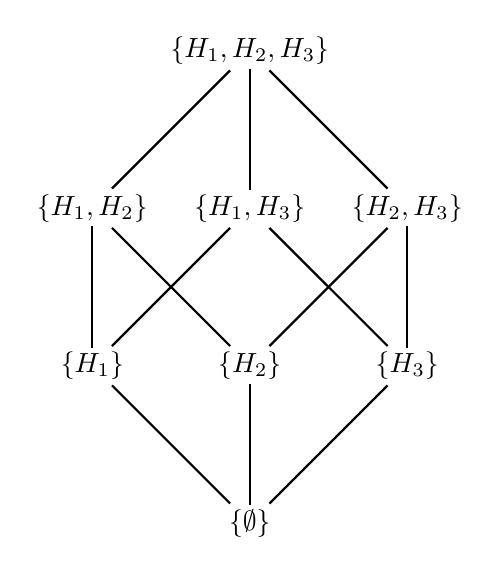
\begin{tikzpicture}
    % First, locate each of the nodes and name them
        \node (top) at (0,0) {$\{H_1, H_2, H_3\}$};
        \node (left) at (-2, -2) {$\{H_1, H_2\}$};
        \node (center) at (0, -2) {$\{H_1, H_3\}$};
        \node (right) at (2, -2) {$\{H_2, H_3\}$};
        \node (one) at (-2, -4) {$\{H_1\}$};
        \node (two) at (0, -4) {$\{H_2\}$};
        \node (three) at (2, -4) {$\{H_3\}$};
        \node (empty) at (0, -6) {$\{\emptyset \}$};

    % Now draw the lines:
        \draw [thick, shorten <=-2pt, shorten >=-2pt] (top) -- (left);
        \draw [thick, shorten <=-2pt, shorten >=-2pt] (top) -- (center);
        \draw [thick, shorten <=-2pt, shorten >=-2pt] (top) -- (right);
        \draw [thick, shorten <=-2pt, shorten >=-2pt] (left) -- (one);
        \draw [thick, shorten <=-2pt, shorten >=-2pt] (left) -- (two);
        \draw [thick, shorten <=-2pt, shorten >=-2pt] (center) -- (one);
        \draw [thick, shorten <=-2pt, shorten >=-2pt] (center) -- (three);
        \draw [thick, shorten <=-2pt, shorten >=-2pt] (right) -- (two);
        \draw [thick, shorten <=-2pt, shorten >=-2pt] (right) -- (three);
        \draw [thick, shorten <=-2pt, shorten >=-2pt] (one) -- (empty);
        \draw [thick, shorten <=-2pt, shorten >=-2pt] (two) -- (empty);
        \draw [thick, shorten <=-2pt, shorten >=-2pt] (three) -- (empty);
    \end{tikzpicture}   
    \caption{A Hasse Diagram for a world with 3 possible states.}
    \label{fig:hesse}
\end{figure}

This paradigm allows an agent to have a probability over each of the $n$ possible states in this world. This forms the basis of an agent's opinion, also referred to as a set of beliefs. These opinions can be combined with those of other agents in a variety of different ways. Thus, it becomes possible to assign a probability mass to each of the sets shown in \cref{fig:hesse} denoting the perceived likelihood of that set including the true state of the world. One of the axioms of this framework is that $P(W) = 1$, which intuitively makes sense as it must be the case that at least one of these states is true, although knowing this fact does not enlighten anyone who learns it. $P(\emptyset) = 0$ is equally informative. 

In published research, there are two prominent ways that agents share their full set of beliefs. The first involves each agent holding a set of beliefs over the state of the world, with a variable that alters the perceived reliability of each other agent individually, $\alpha_k$~\cite{Hegselmann2002Opinion}. At each moment in time, an agent $i$ averages together the opinions of all of its peers weighted by the reliability of each other agent in the population $\alpha_{k}, k \neq i$  to form its updated opinion $x(t+1)$. This seemingly simple model can produce some impressive dynamics, showing that just a few agents are key nodes in the social fabric of this population and that they have a disproportionate influence on the convergence of the system, though this is challenging to demonstrate analytically. Other similar models include~\cite{Deffuant2000MixingAgents}, \cite{Proskurnikov2017OpinionAgents} and~\cite{Friedkin1999SocialChange}. The Friedkin and Johnsen (FJ) model provides the closest analogue to the approach here taken, though different in that it is used to consider the effects of prejudice in the population. Importantly, the FJ model does include an element of an agent's past beliefs, which seems to be a logical inclusion. There is experimental evidence to suggesting there is some validity to the FJ model as it was tested on 50 groups of 4 students verifying that a more influential member of a population tended to emerge~\cite{Friedkin2011APower}. These experiments were constructed such that four students were in separate rooms faced with reaching a collective decision. They were able to make as many phone-calls to any other member of the group and had 20 minutes in which to make their decision. The emergent behaviour showed that generally a single member of the group quickly dominated the decision making process, revealing themselves as the most influential node in this artificial social network. 

A second approach is to consider the population with an outside perspective. In this model, a subset of the population is selected at random and ``pooled'' together, combining their opinions together at each timestep~\cite{Degroot1974ReachingConsensus, Lee2018CombiningConsensus}. This proposition allows for a variety of pooling operators that can affect the eventual collective decisions of the population. The methods proposed originally by DeGroot~\cite{Degroot1974ReachingConsensus} involve a linear combination of beliefs of the agents in a pool, though the models of Lee, Lawry and Winfield introduce nonlinear models that demonstrate aptitude at reaching a consensus under a variety of different possible circumstances. These pooling methods incorporate a generalisation of the idea ``two-heads-are-better-than-one'' as, in theory, the more individuals involved in the decision, the more information is likely to be available. In an anthropoid context, this phenomenon is also referred to as ``the wisdom of the crowd'' though there is some dispute as to its merits. It is assumed that $n$ individuals contain at least as much information as just one, but by the same token, the $n$ individuals contain at least as much misinformation~\cite{Dalkey1963AnExperts}. There is similar experimental evidence to support these pooling methods in a managerial technique referred to as the Delphi Method, despite being hardly oracular. Under this scheme, a panel of experts are gathered to reach a collective decision. They each answer a number of questions while isolated from one another. Then they are each presented with a summary of the responses from their peers and invited to update their own responses. This process is repeated until a predetermined condition is met~\cite{Dalkey1963AnExperts}. 

A common thread in the previous two methods is the combination of the agents full set of beliefs. Since this is not the method by which humans approach decisions, this report seeks to provide an insight into various methods by which only a subset or the most salient and persuasive information need be shared between agents in a simulated population~\cite{Harvey2019QuantitativeMarking}. With such an insight, it could become simpler to explain how a population of agents reach a certain decision, or persuade an agent with an erroneous set of beliefs too complex to change manually. This report aims to take a preliminary step in understanding aspects of the nuanced phenomenon of persuasion.

\Cref{sect:method} will outline the experimental set up for the models that will be described in \cref{sect:speaker_models}. The following section shall discuss the results found before suggesting a number of extensions to \cref{sect:speaker_models} that aim to more closely mimic anthropomorphic behaviours that incorporate aspects of persuasion. 



\section{Models}\label{sect:method}
\lhead{\textit{Models}}

As previously alluded to in \cref{fig:hesse}, the models that follow rely on an opinion being formed of a probability mass being assigned to a set of possible worlds. For illustrative purposes, consider the $3$ dimensional case above. The opinion of an agent at time $t$ can then be represented in a vector of the form:

\begin{center}
$P^t = \begin{bmatrix}
    p_{1}\\
    p_{2}\\
    p_{3}
\end{bmatrix}$
\end{center}

where $P_i$ reflects the probability mass placed by the agent in question upon state $s_i$. By the axiom $P(W) = 1$, the vector $P^t$ must also sum to $1$. This allows us to form a right-stochastic matrix\footnote{A right stochastic matrix is defined as a square, non-negative matrix for which the rows sum to $1$~\cite{Gagniuc2017MarkovExperimentation}.}, representing the collective beliefs over $n$ states of the world of the full population of $K$ agents at time $t$:

\begin{center}
$\mathbf{P}^t = \begin{bmatrix}
    P_{11} & P_{12} & P_{13} & \dots  & P_{1n} \\
    P_{21} & P_{22} & P_{23} & \dots  & P_{2n} \\
    \vdots & \vdots & \vdots & \ddots & \vdots \\
    P_{K1} & P_{K2} & P_{K3} & \dots  & P_{Kn}
\end{bmatrix}$
\end{center}

Each of the $K$ agents is initialised with $n$ distinct beliefs computed by drawing $n-1$ numbers on the interval $ [ 0,1 ] $. These numbers are sorted and the interval between them yields the initial set of beliefs $P_{k}^0$. In the $3$-dimensional case, at any given time, the beliefs of an agent can be represented as a point on the blue surface in \cref{fig:3d-simplex}. This can be projected down to a $2$-dimensional plot such as those shown as shown in~\cref{fig:2d-simplex}.  In this plot, an agent in the corner of the triangle could be described as being certain, extremist, or having a strong belief in a single hypothesis. Alternatively, those more toward the centre have a relatively uniform distribution in probability space and so would be uncertain or have a weak belief.  

\todo{Correct the vertex labels on this plot}
\begin{figure}
\begin{minipage}[ht]{0.45\textwidth}
    \centering
    \resizebox{\linewidth}{0.74\linewidth}{
   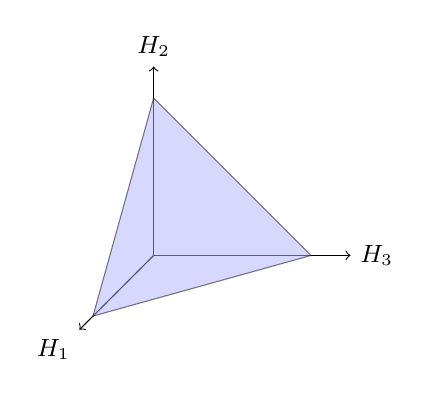
\begin{tikzpicture}[line join = round, line cap = round]
\coordinate [] (A) at (2,0,0);
\coordinate [] (B) at (0,0,2);
\coordinate [] (C) at (0,2,0);
\coordinate [] (D) at (0,0,0);

\draw[->] (0,0) -- (2.5,0,0) node[right] {\small $H_3$};
\draw[->] (0,0) -- (0,2.4,0) node[above] {\small $H_2$};
\draw[->] (0,0) -- (0,0,2.45) node[below left] {\small $H_1$};
\foreach \i in {A,B,C,D}
    \draw[dashed] (0,0)--(\i);
\draw[-, fill=blue!30, opacity=.5] (A)--(B)--(C)--cycle;
\end{tikzpicture} }
\subcaption{$3$-dimensional simplex}\label{fig:3d-simplex}
\end{minipage}
\hfill
  \begin{minipage}[ht]{0.45\textwidth}
    \includegraphics[width=\textwidth]{Images/Figures/OpenModel/open_model_BC_n_3_p_100_gullibility_0,3_runs_10.png} 
    \subcaption{$2$-dimensional projection}\label{fig:2d-simplex}
 \end{minipage}
\caption{An example of a $3$-dimensional simplex over a world with $3$ possible states, projected down to $2$-dimensions. } 
\end{figure}

Once the population is initialised, the lanes of communication must be described. Parker and Zhang describe a characteristic of their model they name the ``well-stirred'' assumption. This assumes that the population is sufficiently mixed together that it is acceptable to select agents at random. This can be thought of in a similar way to the social lattice described in~\cite{Deffuant2000MixingAgents}, though instead of a simple square lattice, the network is fully connected with communicating pairs selected at random. Two agents are drawn randomly from the population, one to be the speaker, one to be the listener. This model is based on a special case of the convention set out by~\cite{Lewis2002ConventionStudy}. This work describes a communicator that acts in its best interests to convey a message that reflects a state of the world that it perceives to be true. This communicator broadcasts its message to an audience that in our case is only one agent but could be generalised to many and, subsequently, the audience performs an action based on the communication it receives. In our case, this is represented in \cref{fig:simple_interaction}. The communication created by the speaker is an argument it hopes will persuade the listener to take some action that will update its beliefs to more closely align to the speaker's. 

 \begin{figure}[H]
 	\centering
 	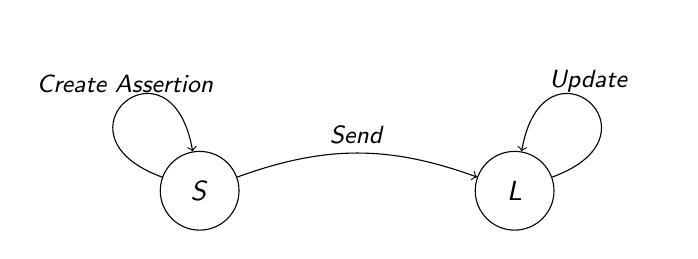
\begin{tikzpicture}[baseline=(S.base)]
 		\tikzset{every loop/.style={min distance=10mm,looseness=10}}
 		\node (S) at (0, 0) [shape=circle,draw,minimum size=1cm] {\textit{S}};
 		\node (L) at (4, 0) [shape=circle,draw, minimum size=1cm] {\textit{L}};
 		\path[->] (S) edge[bend left = 20] node[above]{\small \textit{Send}} (L)
 		edge[loop above,in=100,out=160, min distance=8mm,looseness=8] node{\small \textit{Create Assertion}} (S)
 		(L) edge[loop above,in=80,out=20, min distance=8mm,looseness=8] node{\small \textit{Update}} (L);
 	\end{tikzpicture}
 	\caption{Simple model of the interaction between two agents. \textit{S} is the speaker and \textit{L} is the listener. \textit{S} creates an argument that it then sends to \textit{L}. \textit{L} may then update its own beliefs according to the argument it receives from \textit{S}.}
 	\label{fig:simple_interaction}
 \end{figure}
 
Initially, it is assumed that the speaker will be aware of the listener's opinions prior to communicating the argument and how the listener will react upon hearing it. This process is repeated iteratively until either we reach the maximum number of iterations or the system can be said to have converged, as defined in~\cref{eq:shannon_entropy}. It is the aim of the speaker to share its opinion on the states of the world it believes to be true with the listener in the hopes that the listener will change its attitude to more closely resemble that of the speaker. 



\begin{algorithm}[H]
\SetAlgoLined
\KwResult{Simulation of agent based communication }
 initialization\;
 \While{$i < t_{max}$}{
  selectSpeaker\;
  selectListener\;
  speakerConstructArgument\;
  listenerReactToArgument\;
  \eIf{Converged}{
   break\;
   }{
   i++\;
  }
 }
 \caption{Method}
\end{algorithm}

There are several features that can be useful in determining the dynamics of this system. The average entropy of the population as a whole denotes the level to which the agents have become certain in a single state~\cite{Shannon1948ACommunication}. This is defined as

\begin{equation}\label{eq:shannon_entropy}
    \hat{E}^t = \frac{1}{K} \sum_i^K - \mathbf{P}^t_i \cdot \log ( \mathbf{P}^t_i)
\end{equation}

The system is said to have converged when the entropy has not changed by more than $\eta $ for $T$ iterations, expressed as $\Delta \hat{E}^T = \abs{ \hat{E}^t -  \hat{E}^{t+T}}  \leq \eta$. However, entropy only highlights whether or not the agents hold strong beliefs, not that they agree on those beliefs. Hence, the J-Divergence is used as a symmetric version of KL-Divergence, used to determine the average distance between all pairs of agents in probability space~\cite{Johnson2001SymmetrizingDistance}. It is defined as

\begin{equation}
    \hat{J}_{t} = \frac{1}{K} \sum_j^K \frac{1}{K} \sum_i^K  \frac{1}{2} \left( \mathbf{P}^t_i \log \left( \frac{ \frac{1}{2} (\mathbf{P}^t_i + \mathbf{P}^t_j) }{\mathbf{P}^t_i} \right) +  \mathbf{P}^t_j \log \left( \frac{ \frac{1}{2} (\mathbf{P}^t_i + \mathbf{P}^t_j) }{\mathbf{P}^t_j} \right) \right)
\end{equation}

There are two parts of this model that we will explore. Firstly, we shall consider methods by which a speaker can construct an assertion, increasing in their complexity from openly revealing an agents underlying probability distribution to tailoring the speakers assertion to the listener. Secondly, we define four actions the listener can take, empowering them to react to arguments in a variety of ways, either passively, with discernment or with steadily less and less importance placed on new information as time passes.








\subsection{Communicator behaviours in collective decision-making} \label{sect:speaker_models}
\lhead{\textit{Speaker Models}}

\subsection*{Open Model}

The argument $\mathbf{A}$ that the speaker defines should reflect the underlying set of beliefs in the agent and also produce the desired reaction from the listener~\cite{Lewis2002ConventionStudy}. Since the goal of the speaker is to bring listeners around to its set of beliefs, an intuitive approach might be to simply transmit a complete representation of their set of beliefs at time $t$ to the listener. This requires the speaker to be totally open about the nature of its beliefs, and including them in as an argument  

\begin{equation}
    \mathbf{A} = P_{S}^t
\end{equation}

where $S$ is the index of the speaker. Evidently, this assertion takes the form of an $n$-dimensional vector of numbers on the interval $[0,1]$ that sum to $1$. Consequentially, it is intuitive that a combination of such vectors is unlikely to result in an agent that is any more certain in a single state of the world than they were before. This shall be explored in~\cref{sect:analysis}. One benefit of this model is that it is highly transparent, allowing an observer to precisely track the beliefs of the population as they evolve. 


\subsection*{Bottom Up Model}

The models hereafter are less revealing, allowing the speaker to communicate a set of worlds it believes to be possible, rather than its distribution over them. Consider \cref{fig:hesse}. An agent practising the Bottom Up approach, as intimated by the name, defines its assertion by considering the bottom layer of the Hasse diagram. Any state $j$ for which the agent $i$ has sufficiently high probability $P_{i,j}$ is included in the assertion. More formally, 

\begin{equation}
    \mathbf{A} = \{ H_j: P_{ij} > \gamma  \}
\end{equation}

where $H_j$ represents the $j^{\textnormal{th}}$ state of the world and $\gamma$ is a threshold on the interval $[0,1]$ constant for all agents. Practically, $\mathbf{A}$ can be viewed as a $1 \times n$ binary membership vector given by applying an indicator function to the asserted set. This model shields the internal beliefs of the speaker while only allowing it to put forward assertions it believes to be true to a certain level. It should be noted, however, that for values of $\gamma > 0.5$, the speaker can only assert a set containing only one element, hereafter referred to as a singleton. This is the most precise assertion that can be made as both $\emptyset$ and $W$ reveal nothing as it is equivalent to arguing ``I believe nothing to be true'' or ``I believe the true state to be possible'', neither of which contribute anything new to a discussion. 

An interesting feature of this model is that, for $\gamma > \frac{1}{n}$, a region of probability space exists in which it is not possible for an agent to create a meaningful assertion. Take, for example, $\gamma = 0.4, n=3$. It is possible that there exists an agent at time $t$ that is selected as speaker with a set of beliefs

\begin{center}
    
$P^t_L = \begin{bmatrix}
    0.35\\
    0.35\\
    0.3
\end{bmatrix}.$
\end{center}

This can create possible distributions of the population for which the agents are incapable of speech, creating a mute population necessarily at a steady state. 

\subsection*{Top Down Model}

As its name suggests, the following model adopts an opposite approach to the Bottom Up method. In this example, the agent constructs its argument starting from the top of \cref{fig:hesse}, iteratively whittling away elements of the set $\mathbf{W} = \{H_1, H_2, \dots, H_n  \}$ for which the probability is lowest. The agent will compute its own probability in the argument $\mathbf{A}$ by summing the probabilities of the states within the set. If this sum is above a threshold $\gamma$ then the agent will broadcast the argument. Otherwise it will remove the element which associated with the minimum probability in its set of beliefs. \Cref{alg:TD} outlines the methodology in more detail. This approach can be written as


\begin{equation}
    \mathbf{A} = \{ H_j: P(\mathbf{H}) > \gamma  \},
\end{equation}

where $\gamma$ is again a threshold kept constant across all agents, $H_j$ is the $j^{\textnormal{th}}$ possible state of the world, and $P(\mathbf{H})$ is the probability of the set of states $\mathbf{H}$, where $\mathbf{H}$ is obtained by the method described above.

\begin{algorithm}[H]
\SetAlgoLined
\KwResult{Argument $\mathbf{A}$ }
 $p = P(W)$\;
 $\mathbf{A} = W$\;
 $i=1$\;
 \While{$i < n$}{
  $S_{min} \gets min(p_i)$\;
  $\mathbf{A} \gets \mathbf{A} \setminus \{S_{min}\}$\;
  $p = P(\mathbf{A})$\;
  \eIf{$p \leq \gamma$}{
   return $\mathbf{A}$\;
   }{
   i++\;
  }
 }
 return $\mathbf{A}$\;
 \caption{Top Down Model} \label{alg:TD}
\end{algorithm}


This method aims to whittle the assertion $\mathbf{A}$ down to the most precise set of possible worlds that still seems plausible to the speaker. The speaker can only state things it believes to be true. It is important to note, however, that the significance of $\gamma$ differs between the Top Down and the Bottom Up model. In the latter, it is a threshold that only applies to individual states whereas the former accounts for sets of states instead. This means that care must be taken in making direct comparisons between the models. 


\subsection*{Optimised Model}

Thus far, the speakers in previous models have failed to make use of one valuable piece of information. They do not consider the beliefs of the listener in the construction of their arguments. This final model rectifies this lapse. 

In this world, all agents have perfect information; they know the beliefs of every other agent as well as how they may react to hearing new pieces of information (an assumption that will be altered later). It is therefore practical for the speaker to devise the best possible argument for each and every speaker. The best outcome for the speaker is for the listener to update their set of beliefs to be as close to the speakers' as possible and hence, minimise the J-Divergence between the two. This can be posed as the following unconstrained Integer Programming optimisation problem

\begin{equation}
    minimise \hspace{1.2em} z = \frac{1}{2} \left( P^t_S \log \left( \frac{ \frac{1}{2} (P^t_S + P^{t+1}_L(\mathbf{A})) }{P^t_S} \right) +  P^{t+1}_L(\mathbf{A}) \log \left( \frac{ \frac{1}{2} (P^t_S + P^{t+1}_L(\mathbf{A})) }{P^{t+1}_L(\mathbf{A})} \right)     \right),
\end{equation}

where $P_S$ and $P_L$ are the speaker and listeners beliefs respectively and $P_L^{t+1}$ is a function of the argument $\mathbf{A}$ that the speaker broadcasts. This system empowers the speaker to make any argument it needs to in order to convince the listener, regardless of the speakers own opinions. It would be simple to introduce an integrity constraint, restricting the speaker to only arguments it believes itself, but it is worth investigating the effects of allowing an agent total freedom in its arguments. 





\subsection{Audience behaviours in the collective decision-making process} \label{sect:listener_models}

\subsection*{Simple Listener Model}
Having addressed multiple ways for the speaker to construct an argument, it is imperative to define the strategies that listener agents may employ to update their attitudes. Drawing inspiration from the Friedkin and Johnsen model~\cite{Friedkin1999SocialChange}, we define an update rule that maintains an element of the agents previous beliefs as well as assimilating the new information. 

The equation we will use shall be


\lhead{\textit{Listener Models}}
\begin{equation} \label{eq:BU_update_rule}
    \mathbf{P}^{t+1}_L = \alpha \cdot \mathbf{P}^{t}_L + (1 - \alpha) \cdot  \frac{\mathbf{A} \odot \mathbf{P}^t_L}{\mathbf{A} \cdot \mathbf{P}^t_L}
\end{equation}

where $\alpha$ is a parameter on the interval $[0, 1]$ that governs the susceptibility of an agent to new information~\cite{Hegselmann2002Opinion}. In Hegselmann's work this parameter differs depending upon how reliable the listener believes the other agent to be, while, here, it is constant across all agents. Finally, $\odot$ denotes the elementwise or Haramaard product~\cite{Johnson1990MatrixApplications}. The last component of this equation serves to condition the speaker's argument $\mathbf{A}$  on the listener's original beliefs and then renormalise this such that the agent's probability distribution remains valid by summing to $1$. Any agent whose set of beliefs loses this property is described as incoherent and withdrawn from the population~\cite{Lee2018CombiningConsensus}. Furthermore, it is important to manage the listeners use of this update equation as, in the case where the cardinality of the set $\mathbf{A}$, $|\mathbf{A}| = 0$ \cref{eq:BU_update_rule} is undefined. In this case, the listener simply will not update.  

It should be noted that the Open Model represents a special case. The above equation is tailored toward arguments of binary vectors so if the Open Model is applied the equation becomes 

\begin{equation} 
    \mathbf{P}^{t+1}_L = \alpha \cdot \mathbf{P}^{t}_L + (1 - \alpha) \cdot \mathbf{A} 
\end{equation}


\subsection*{Discerning Model}

The previous model deprives the listener agent of the ability to disregard any information it receives; it will always update its beliefs based on new information. In order to address this, the model requires that when the listener reverses the process used to create the argument on its own beliefs, the same condition must be met. This is only possible in the Bottom Up and Top Down models as they involve a specified criterion that the argument must meet to be transmitted. Consider the following example for illustration. 

Let the speaker broadcast \hspace{10em}

\begin{minipage}[ht]{0.45\textwidth}
\begin{center}
$\mathbf{A} = \begin{bmatrix}
    1\\
    0\\
    1
\end{bmatrix}$
\end{center}
\end{minipage}
and let
\begin{minipage}[ht]{0.45\textwidth} 
$P^t_L = \begin{bmatrix}
    0.6\\
    0.15\\
    0.25
\end{bmatrix}$
\end{minipage}

In the case that this argument is constructed with the Bottom Up method with a threshold $\gamma = 0.4$, the listener compares the argument with its own beliefs. It finds that $p_1 > \gamma$ passing the requirement, $p_2$ is not asserted so is not considered, and finally $p_3 < \gamma$. Since the assertion of $H_3$ seems unlikely to the agent, it rejects the assertion outright, refusing to update. Similarly, if the argument is created with the Top Down model with a threshold $\gamma = 0.8$, then the listener takes the dot product of $\mathbf{A}$ and $P_L^t$. In this case this returns a value of $0.85$ which is greater than $\gamma$ so the listener accepts the argument and updates accordingly. 


\subsection*{Spiteful Model}

The previous model is relatively passive in the sense that, should it disagree with the argument, it does not update its beliefs whatsoever. However, anyone who has ever been told to ``calm down'' while irate can likely attest that occasionally an argument can often backfire if the listener finds it incredible. In this model, the criteria for disagreeing with an argument are as above, but, instead of passively ignoring the assertion, the listener will update using $\mathbf{A}^c$.

It is expected that both the Discerning and Spiteful models will cause divisions in the population, creating regions in which agents are incapable of responding to an argument. 



\subsection*{Stubborn Model}

The final listener model aims to mimic the growth of stubbornness as time progresses. In this model, $\alpha$ from \cref{eq:BU_update_rule} is a function of the number of arguments the agent has received, henceforth given by $\tau$. The equation is

\begin{equation}
    \alpha = 1 - (1 - \alpha_0) e^{-\lambda \tau}
\end{equation}

where $\alpha_0$ is the initial value of $\alpha$ and $\lambda = \frac{K}{t_max}$ is a rate at which the agents become stubborn. This allows an agent to be strongly influenced by the early arguments it hears but then, as it hears more and more, come to rely more heavily on its previous beliefs. This can be seen in \cref{fig:stubbornness_curve}. 


\begin{figure}[H]
    \centering
    \includegraphics[width=0.49\textwidth]{Images/Misc/Stubbornness.png}
    \caption{A graph to show the rate at which agents change the importance they place on new information in the Stubborn Model. \textit{Using $\alpha_0 = 0.3, \lambda = 0.01$}}
    \label{fig:stubbornness_curve}
\end{figure}
\chapter{Analysis}\label{sect:analysis}

\section{Fixed Points Analysis} \label{sect:fixed_point_analysis}

All of the models in the previous chapter represent discrete time mappings. As such, it is therefore possible to identify fixed points so as to better understand the behaviour of some of the models. As in~\cite{Hegselmann2002OpinionSimulation}, it is challenging to provide analytical insights for some combinations of these models. However, the Open model can be readily analysed with Passive listeners.


For a fixed point in this system, it must hold that $\underline{\underline{\mathbf{P}}}^{t+1} = \underline{\underline{\mathbf{P}}}^t$. This equation requires that no agent has updated its beliefs and so the system is unchanged. The structure of the method defined at the beginning of~\cref{sect:method} dictates that at most one listener agent will update at any one iteration. Hence, at most only one row of matrix $\underline{\underline{\mathbf{P}}}^t$ will change and so can be considered in isolation. 

Without loss of generality, let us select two agents from $\underline{\underline{\mathbf{P}}}^t$ and label them $\underline{\mathbf{P}}_s$ and $\underline{\mathbf{P}}_l$ respectively. Hence, for all agents, a fixed point must satisfy

\begin{equation}
    \underline{\mathbf{P}}_l = \alpha \cdot \underline{\mathbf{P}}_l + (1 - \alpha) \cdot \underline{\mathbf{P}}_s. \label{eq:open_FP}
\end{equation}

There are two possible ways this can occur. Firstly, when $\alpha = 1$, we have a trivial fixed point. Secondly, assuming $\alpha < 1$, the fixed point occurs when $\underline{\mathbf{P}}_l=\underline{\mathbf{P}}_s$ for all possible pairs of agents. This reveals that it is likely that a fixed point will be found when the agents have converged to a single shared belief, a claim that is supported in simulation. To test the stability of these fixed points, we take the eigenvalues of the Jacobian of \cref{eq:open_FP} which gives $\alpha \underline{\underline{\mathbf{I}}}$. The system is stable when the modulus of all of the eivengalues lie within the unit circle. The trivial fixed point is clearly stable as $\abs{\alpha} = 1$. The non-trivial fixed point $\underline{\mathbf{P}}_l=\underline{\mathbf{P}}_s$ is asymptotically stable as $\abs{\alpha} < 1$. This shows that, under this particular scheme, the agents are guaranteed to cluster together, converging upon a consensus. However, the existence of a stable fixed point does not guarantee that the population converges to a belief with absolute certainty. 

Perhaps more interesting is the case of Bottom Up speakers and Passive listeners. Using the same notation as above, the equation to reveal fixed points becomes

\begin{equation}
    \underline{\mathbf{P}}_l = \alpha \cdot \underline{\mathbf{P}}_l + (1 - \alpha) \cdot \frac{\underline{\mathbf{A}} \odot \underline{\mathbf{P}}_l}{\underline{\mathbf{A}} \cdot \underline{\mathbf{P}}_l}. \label{eq:BU_FP}
\end{equation}

From this equation, it can be shown that there are three fixed points. The first is trivial at $\alpha = 1$. The second occurs when $P_L(\mathbf{A}) = 0$ meaning that the listener has a $0$ probability for every state that the speaker has asserted and so does not update. The third occurs when $P_L(\mathbf{A}) = 1$, meaning that the speaker has asserted at least every state for which the listener has a non-zero probability. This final fixed point indicates that

\begin{align*}
    \underline{\mathbf{P}}_l = \frac{\underline{\mathbf{A}} \odot \underline{\mathbf{P}}_l}{\underline{\mathbf{A}} \cdot \underline{\mathbf{P}}_l}.
\end{align*}

This condition highlights two things: firstly, that $ \underline{\mathbf{A}} \cdot \underline{\mathbf{P}}_l = 1 $; secondly, that $ \underline{\mathbf{A}} \odot \underline{\mathbf{P}}_l =  \underline{\mathbf{P}}_l$. These are equivalent to $\sum^n_j A_j p_{l,j} = 1$ and $ p_{l,j} = A_j p_{l,j} $ respectively. 

As previously, to show the stability of these fixed points, the Jacobian must be computed. First, consider the diagonal elements of $\underline{\underline{\mathbf{J}}}$, given by

\begin{align}
    J_{a,a} = \frac{d f(p_{l,a})}{d p_{l,a}} &= \frac{d}{d p_{l,a}} \left( \alpha p_{l,a} + (1 - \alpha) \cdot \frac{A_a p_{l,a}}{\sum^n_j A_j p_{l,j}} \right) \\
    &= \alpha + (1 - \alpha) \cdot \left( \frac{A_a}{\sum^n_j A_j p_{l,j}} - \frac{A_a^2 p_{l,a}}{\sum^n_j A_j p_{l,j}} \right) \\
    &= \alpha + (1 - \alpha) \cdot \frac{A_a}{\sum^n_j A_j p_{l,j}} \left( 1 - \frac{A_a p_{l,a}}{\sum^n_j A_j p_{l,j}} \right), \\ 
\end{align}

and off-diagonals are given by

\begin{align}
    J_{a,b} = \frac{d f(p_{l,a})}{d p_{l,b}} &= \frac{d}{d p_{l,b}} \left( \alpha p_{l,a} + (1 - \alpha) \cdot \frac{A_a p_{l,a}}{\sum^n_j A_j p_{l,j}} \right) \\
    &= 0 + (1 - \alpha) \cdot \left( - \frac{A_a p_{l,a} A_b}{\sum^n_j A_j p_{l,j}} \right). \\
\end{align}


When $\alpha = 1$, it can be seen that off-diagonals are $0$, and the diagonal elements are $1$, therefore the eigenvalues of $\underline{\underline{\mathbf{J}}}$ are $1$. When $P_L(\mathbf{A}) = 0$, the diagonal elements of $\underline{\underline{\mathbf{J}}}$ are $\alpha$, however, the off-diagonals are not so clear. Consider the full $n \times n$ real matrix

\begin{center}
$\underline{\underline{\mathbf{J}}} = \begin{bmatrix}
    \alpha - (1 - \alpha) A_1 (1- p_{l,1}) & - (1 - \alpha) A_1 p_{l,2} & \dots  & -(1 - \alpha) A_1 p_{l,n} \\
    - (1 - \alpha) A_2 p_{l,1} &  \alpha - (1 - \alpha) A_2 (1- p_{l,2}) &  \dots  & -(1 - \alpha) A_2 p_{l,n} \\
    \vdots & \vdots & \ddots & \vdots \\
    - (1 - \alpha) A_n p_{l,1} & - (1 - \alpha ) A_n p_{l,2} &  \dots & \alpha - (1 - \alpha) A_n (1- p_{l,n}) \\

\end{bmatrix}$.
\end{center}

For stability, the modulus of the eigenvalues of this matrix must lie within the unit circle, however, it is not possible to evaluate each eigenvalue in the general case for $n>5$, due to the Abel-Ruffini Theorem~\cite{Abel1824MemoireDegre}. With some minor manipulations to this matrix, it is possible to apply Perrón-Frobenius theorem to calculate the largest positive real eigenvalue, but this is insufficient for determining the stability, as there is no guarantee that all the eigenvalues are real~\cite{Perron1907ZurMatrices}. Fortunately, Gershgorin Circle Theorem provides a method for bounding the location of the eigenvalues in the complex plane~\cite{Gerschgorin1931UberMatrix}. This theorem states that each eigenvalue $\lambda_a$ of an $n\times n$ square matrix $\underline{\underline{\mathbf{M}}}$ will lie within at least one Gershgorin Disc $D(m_{a,a}, R_a)$ where the centre of the disc $m_{a,a}$ is the $a^\textnormal{th}$ element on the diagonal of $\underline{\underline{\mathbf{M}}}$, and its radius $R_a = \sum^n_{b \neq a}\abs{m_{a,b}}$. Consider \cref{fig:gershgorin}. This figure shows the unit circle in the complex plane and three Gershgorin Discs. If all of the discs were within the unit circle, our system would be stable. It should be noted that, because the eigenvalues must lie within at least one of these discs, having a disc outside the unit circle is a necessary but not sufficient condition for determining that the system is unstable. \\


\begin{figure}
\begin{center}
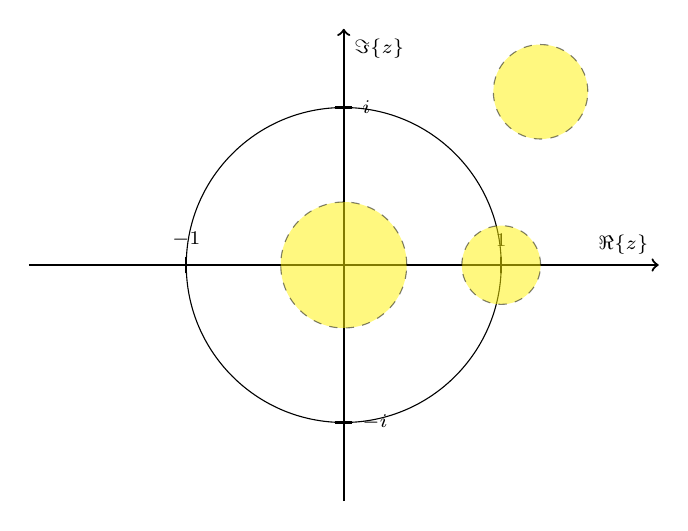
\begin{tikzpicture}
     \begin{scope}[thick,font=\scriptsize]
     % Axes:
     % Are simply drawn using line with the `->` option to make them arrows:
     % The main labels of the axes can be places using `node`s:
     \draw [->] (-4,0) -- (4,0) node [above left]  {$\Re\{z\}$};
     \draw [->] (0,-3) -- (0,3) node [below right] {$\Im\{z\}$};
 
     % Axes labels:
     % Are drawn using small lines and labeled with `node`s. The placement can be set using options
     \iftrue% Single
     % If you only want a single label per axis side:
     \draw (2,-3pt) -- (2,3pt)   node [above] {$1$};
     \draw (-2,-3pt) -- (-2,3pt) node [above] {$-1$};
     \draw (-3pt,2) -- (3pt,2)   node [right] {$i$};
     \draw (-3pt,-2) -- (3pt,-2) node [right] {$-i$};
     \else% Multiple
     % If you want labels at every unit step:
     \foreach \n in {-4,...,-1,1,2,...,4}{%
         \draw (\n,-3pt) -- (\n,3pt)   node [above] {$\n$};
         \draw (-3pt,\n) -- (3pt,\n)   node [right] {$\n i$};
     }
     \fi
     \end{scope}
     % The circle is drawn with `(x,y) circle (radius)`
     % You can draw the outer border and fill the inner area differently.
     % Here I use gray, semitransparent filling to not cover the axes below the circle
     \path [draw=black] (0,0) circle (2);
     \path [draw=black, dashed, fill=yellow, semitransparent] (0,-0) circle (0.8);
     \path [draw=black, dashed, fill=yellow, semitransparent] (2,0) circle (0.5);
     \path [draw=black, dashed, fill=yellow, semitransparent] (2.5,2.2) circle (0.6);
     % Place the equation into the circle:
\end{tikzpicture}
\end{center}
\caption{A plot of an Argand diagram demonstrating Gershgorin Circle Theorem. The system is stable if the eigenvalues are all within the unit circle, shown in black. The yellow circles show Gershgorin discs of a system. The theorem dictates that each eigenvalue must lie within at least one of these discs. }
\label{fig:gershgorin}
\end{figure}

Therefore, for the fixed point $P_L(\mathbf{A}) = 0$, the eigenvalues lie within Gershgorin Discs of the form 

\begin{align}
    &D(\alpha, \sum_{b \neq a}^n \abs{ - (1 - \alpha) A_a p_{l,b} } ) \nonumber \\
    &D(\alpha, \sum_{b \neq a}^n (1 - \alpha) A_a p_{l,b} ) \nonumber \\
    &D(\alpha, (1 - \alpha) A_a (1 - p_{l,a}) ) .
\end{align}

Here, as $\underline{\mathbf{A}}$ is a binary vector, this equation can be broken down into two cases. Firstly, let $A_a = 0$. In this case, the disc becomes $D(\alpha, 0)$, which is within the unit circle. Secondly, let $A_a = 1$. In this case, $p_{l,a} = 0$, and therefore the disc becomes $D(\alpha, 1-\alpha)$, which makes contact with, but does not cross, the unit circle. Hence, for $P_L(\mathbf{A}) = 0$, the fixed point is stable. 

A similar argument exists for the fixed point at $P_L(\mathbf{A}) = 1$. Here, the eigenvalues of $\underline{\underline{\mathbf{J}}}$ must lie within discs of the form 

\begin{align}
 D(\alpha - ( 1 - \alpha ) A_a ( 1 - p_{l,a}), \sum_{b \neq a}^n \abs{ - (1 - \alpha) A_a p_{l,b} }) \nonumber\\
 D( \alpha - (1 - \alpha) A_a (1 - p_a), (1 - \alpha) A_a (1 - p_{l,a})).  
\end{align} \label{eq:2FPGershgorin}

As $\underline{\mathbf{A}}$ is a binary vector, we can split~\cref{eq:2FPGershgorin} into two different types of disc, one in which $A_a = 0$ and one in which $A_a = 1$. When $A_a = 0$, the discs are $D(\alpha, 0)$, and so are within the unit circle. When $A_a = 1$, the discs are given by \[ D(\alpha + (1 - \alpha) (1 - p_{l,a}), (1 - \alpha)(1 - p_{l,a})).\] Therefore, the system is stable when \[ \alpha + 2(1 - \alpha)(1 - p_{l,a}) \leq 1.   \]

This simplifies to 
\begin{align}
    \alpha + 2(1 - \alpha) ( 1- p_{l,a}) & \leq 1 \nonumber  \\
    2(1 - \alpha - p_{l,i} + \alpha p_{l,i}) & \leq 1 - \alpha \nonumber\\
    - 2p_{l,a} + 2\alpha p_{l,a} & \leq \alpha - 1 \nonumber \\
    2 p_{l,a} (\alpha - 1) & \leq \alpha - 1 \nonumber \\
    p_{l,a}  & \geq \frac{1}{2}.
\end{align}

Hence, when $A_a = 0$, each corresponding disc is within the unit circle and when $A_a = 1$, the system as a whole is guaranteed to be stable when $p_{l,a} \geq \frac{1}{2}$. This can only happen in one of two ways: $p_{l,a} = 1$ and all other probabilities are $0$, or there are two states for which $p_{l,a} = \frac{1}{2}$. Therefore, it is expected that the system will tend to steady states in which, for every agent, either $p_{l,a} = 1 \textnormal{ or } p_{l,a} = \frac{1}{2}$. Therefore, it is expected that the agents will graduate toward either certainty in a single state of the world, or equal levels of uncertainty in two states. 





\section{Simulation Experiments}

The following experiments were run on an Intel(R) Core i7-8650 CPU 1.90Ghz with the following parameters as default, unless otherwise stated: $n=3, K=100, \alpha = 0.3, \gamma = 0.5, t_{max} = 50,000, \eta = 10^{-5}, T=3$. Error bars are shown at $\pm \sigma$, one standard deviation. 
\subsection{Consensus}

To gain an insight into the dynamics of these systems, let us consider their entropy, as defined in~\cref{eq:shannon_entropy}. This serves as a measure of the uncertainty in the system. High values imply the absence of strong beliefs in the population, and low values imply a level of certainty, though importantly, not consensus. To illustrate the distinction between these entropy values, consider \cref{fig:2d-simplex}. There are some agents in the corners of the Barycenter plot that happen to be initialised with some strong beliefs in some states of the world. These agents will have low entropy values, whereas those closer to the centre of the plot will have much higher entropy values due to their uncertainty. 


\Cref{fig:entropy_all,fig:J-div_all} show plots of entropy and J-divergence changing over time for each of the four models proposed. Here, the listeners are Passive. In can be seen that the entropy and the J-Divergence of the Open model follow significantly different trajectories to the other models. The J-Divergence decreases, as in the other models, although it reaches $0$ almost immediately. This suggests that the agents cluster together rapidly. The entropy plot, however, differs significantly to the other models. It can be seen to increase to a value of $\approx 1.09$. This is approximately the maximum entropy value that could be obtained in a $3$-dimensional world. It is apparent that the agents quickly cluster together, each of them assuming the uniform distribution as their beliefs. This is due to their uniformly random initialisation, not a characteristic of the model. Therefore, the Open model behaves as predicted by~\cref{sect:fixed_point_analysis}, converging to a single point that is approximately the average of every agent's beliefs. It should be noted that there is limited variation in the behaviour of the Open model, as evidenced by the narrow error bars. 

\begin{figure}[H]
 \centering
  \begin{minipage}[ht]{0.49\textwidth}
    \includegraphics[width=\textwidth]{Images/Figures/All/Entropy_25000.png}
    \subcaption{Entropy}\label{fig:entropy_all}
 \end{minipage}
 \hfill
 \begin{minipage}[ht]{0.49\textwidth}
    \includegraphics[width=\textwidth]{Images/Figures/All/J-Div_25000.png}
    \subcaption{J-Divergence}\label{fig:J-div_all}
 \end{minipage}
 \caption{Two plots to show the change in entropy and J-Divergence over time, for the Open, Bottom Up, Top Down, and Optimised models. These plots were obtained using Passive listeners, and were averaged over $100$ runs.}
\end{figure}

The Bottom Up and Top Down models seem to behave indistinguishably, both reducing the uncertainty in the population as time passes, tending toward $0$ at a similar rate for both entropy and J-Divergence. These two approaches are capable of achieving a population of agents that are certain of one state alone. In order to determine whether one is a dominant strategy, the two models must be compared across a variety of different parameter values, explored in the following section.  It should be noted that all models other than the Open model appear to \emph{increase} the disagreement between agents for the first few hundred iterations. This occurs at the same time as the gradient of the entropy plot is maximal. At this time, agents are quickly persuaded toward one particular state, depending on the arguments they hear. Due to the random initialisation, this divides the population, increasing the J-Divergence until a majority forms in support of one possible state and the agents begin to converge toward it. In simulation, this phenomenon manifests in some interesting patterns such as those shown in~\cref{fig:sierpinski_triangle_intro}. 


\begin{figure}[H]
    \centering
    \includegraphics[width=0.45\textwidth]{Images/Figures/Barycenter/Serpinski_example.png}
    \caption{The $500^\textnormal{th}$ iteration of a simulation of the Bottom Up model. $500$ agents are shown, with clusters of agents forming at $\underline{\mathbf{P}}^t_{x} \approx [\alpha, 1-\alpha, 0]^T$. The listeners are Passive. Importantly, the system has not converged at this point.}
    \label{fig:sierpinski_triangle_intro}
\end{figure}

When a listener that has a strong belief in $H_j$ is presented with an assertion $ \mathbf{A} = \{ H_{¬j} \}$, approximately the following update occurs. 


\begin{center}
$\underline{\mathbf{P}}^t_l = \alpha \begin{bmatrix}
    1-\epsilon\\
    \epsilon\\
    0
\end{bmatrix} + (1 - \alpha) \frac{\begin{bmatrix} 0\\1\\0 \end{bmatrix} \odot \begin{bmatrix} 1-\epsilon\\ \epsilon\\ 0 \end{bmatrix}} {\begin{bmatrix} 0\\1\\0 \end{bmatrix} \cdot \begin{bmatrix} 1- \epsilon\\ \epsilon \\ 0\end{bmatrix}} $, \\
\end{center}
where $\epsilon$ is an arbitrarily small positive number, such that $\sum^n_j p^t_{l,j} = 1$. Then 
\begin{center}
$\underline{\mathbf{P}}^t_l =\alpha \begin{bmatrix}
    1 - \epsilon \\
    \epsilon\\
    0
\end{bmatrix} + (1 - \alpha) \begin{bmatrix} 0\\ 1 \\ 0  \end{bmatrix} $ \\

$\underline{\mathbf{P}}^t_l \approx \begin{bmatrix} \alpha \\ 1 - \alpha \\ 0  \end{bmatrix}$.
\end{center}

As an aside, when $\alpha = 0.5$, the plot shows remarkable similarity to the Sierpinski Triangle due to the same phenomenon as~\cref{fig:sierpinski_triangle_intro}, demonstrated in~\cref{fig:sierpinski_compare}. 

\begin{figure}[H]
  \begin{minipage}[t]{0.49\textwidth}
    \includegraphics[width=\textwidth]{Images/Misc/Sierpinski_triangle_real_resized.png}
    \subcaption{Sierpinski Triangle}
  \end{minipage}
  \hfill
 \begin{minipage}[t]{0.49\textwidth}
    \includegraphics[width=\textwidth]{Images/Figures/Barycenter/Serpinski_BU.png}
    \subcaption{Bottom Up Model} \label{fig:sierpinski_BU}
 \end{minipage}
 \caption{ The true Sierpinski Triangle, and the Bottom Up model after $80,000$ iterations with $K=10,000, \alpha=0.5$. The pattern in (b) is not stable and breaks down with time. \textit{Image downloaded from \url{https://bit.ly/2GkoUXI}}  }\label{fig:sierpinski_compare}
\end{figure}


The population in the Bottom Up model forms a particular structure, as shown in~\cref{fig:sierpinski_BU}. The explanation for this structure arises due to the similarity between the update rule and a chaos game. Originally described by Barnsley, a chaos game

\begin{displayquote} 
    ``\dots is a Markov Chain Monte Carlo algorithm that is applied in order to describe probability distributions supported on an attractor of an iterated function system''~\cite{Barnsley2011ChaosSpaces}.
\end{displayquote}

To better understand them, an example of a chaos game is taken from \cite{Feldman.DavidP2012ChaosIntroduction} that bears a resemblance to the general speaker-listener model described in~\cref{sect:method}. In his book, Feldman begins by selecting a point anywhere within the outermost triangle shown in \cref{fig:chaos_game}. Then, if such a device were practical, a three-sided die is rolled, and the point is moved half-way toward the result of the roll. For example, let the first die roll be a $2$. The point would then move to be within the upper shaded triangle, labelled ``$2$''. If the subsequent roll was a $3$, then the point would lie anywhere within the triangle, marked ``$2,3$''. This process can be repeated ad infinitum creating infinitely dense trajectories of this point, as well as revealing areas that it is impossible for the point to reach, shown in white. After an infinite number of iterations, the trajectory of this point will reveal the Sierpinski triangle. Similar results are obtained using the update rule for Passive listeners in which agents update their beliefs towards a vertex that, at least in the early stages of the population's communications, is chosen almost uniformly at random. However, as soon as a large cluster of agents forms, the balance of probability shifts towards them, so the fractal structure of the population begins to break down. In the Optimised model, occasionally the largest cluster can form at a vertex of one of the sub-triangles and remain there, as shown in~\cref{fig:optimised_problem_case}. A further difference is that Passive listeners update towards the vertex by some function $f(\alpha)$, instead of the point moving half-way towards the selected vertex.  

\begin{figure}[H]
\begin{center}
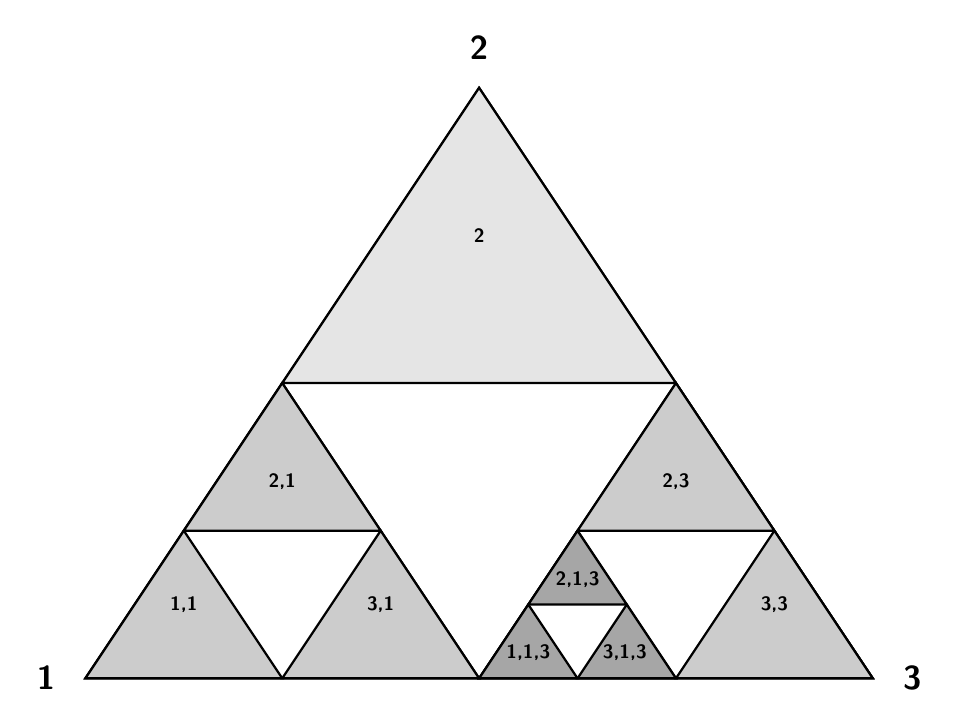
\begin{tikzpicture}
    \draw[thick] (0,0) -- (10,0) -- (5,7.5) -- cycle;
    
    \draw[thick] (0,0) -- (5,0) -- (2.5,3.75) -- cycle;  
    \draw[thick] (10,0) -- (5,0) -- (7.5,3.75) -- cycle;
    \draw[thick, fill=black!10] (2.5,3.75) -- (7.5,3.75) -- (5,7.5) -- cycle;

    
    \draw[thick, fill=black!20] (0,0) -- (2.5,0) -- (1.25,1.875) -- cycle;
    \draw[thick, fill=black!20] (2.5,0) -- (5,0) -- (3.75,1.875) -- cycle;
    \draw[thick, fill=black!20] (1.25,1.875) -- (3.75,1.875) -- (2.5,3.75) -- cycle;
    \draw[thick] (5,0) -- (7.5,0) -- (6.25,1.875) -- cycle;
    \draw[thick, fill=black!20] (7.5,0) -- (10,0) -- (8.75,1.875) -- cycle;
    \draw[thick, fill=black!20] (6.25,1.875) -- (8.75,1.875) -- (7.5,3.75) -- cycle;
    
    
    \draw[thick, fill=black!35] (5,0) -- (6.25,0) -- (5.625,0.9375) -- cycle;
    \draw[thick, fill=black!35] (6.25,0) -- (7.5,0) -- (6.875,0.9375) -- cycle;
    \draw[thick, fill=black!35] (5.625,0.9375) -- (6.875,0.9375) -- (6.25,1.875) -- cycle;

    \node at (5,5.625) {\scriptsize\textbf{2}};
    \node at (5,8) {\large\textbf{2}};
    \node at (-0.5,0) {\large\textbf{1}};
    \node at (10.5,0) {\large\textbf{3}};
    
    \node at (1.25,0.9375) {\scriptsize\textbf{1,1}};
    \node at (2.5, 2.5) {\scriptsize\textbf{2,1}};
    \node at (3.75, 0.9325) {\scriptsize\textbf{3,1}};
    
    \node at (7.5, 2.5) {\scriptsize\textbf{2,3}};
    \node at (8.75, 0.9325) {\scriptsize\textbf{3,3}};
    
    \node at (5.625, 0.32625) {\scriptsize\textbf{1,1,3}};
    \node at (6.25, 1.25) {\scriptsize\textbf{2,1,3}};
    \node at (6.85, 0.32625) {\scriptsize\textbf{3,1,3}};

\end{tikzpicture}
\end{center}
\caption{A pictorial representation of a chaos game to generate a Sierpinski Triangle. A point is chosen at random from the outermost triangle then, at each iteration, is updated half-way towards a randomly selected vertex. The triangle marked ``$3,1,3$'' represents the area that the randomly selected first point must be in if the sequence of vertices has been first $3$, then $1$ then $3$. Repeated ad infinitum will generate a Sierpinski Triangle.}  \label{fig:chaos_game}
\end{figure}

Finally, the Optimised model appears to be failing to live up to its name. While it does induce a reduction in the entropy of the system, it does not enable the agents to become certain that any one state is true. That said, the agents do arrive at a consensus, as evidenced by the J-Divergence plot. This indicates that the agents converge to a single point in probability space, but that that point is not the corner of the Barycenter plot, and thus the agents are not certain in a single state. \Cref{fig:optimised_problem_case} shows a histogram of the final states of agents using the Optimised approach. 

\begin{figure}[H]
    \centering
    \includegraphics[width=0.49\textwidth]{Images/Figures/Optimised/ChaoticAttractorMaybe.png}
    \caption{ A histogram showing the maximum probability at the $25,000^\textnormal{th}$ iteration of the Optimised model, for $100$ runs. It can be seen that there are two main locations the agents converge to, with other, less frequent possibilities in between.  }
    \label{fig:optimised_problem_case}
\end{figure}

\Cref{fig:optimised_problem_case} shows a histogram of $100$ runs at $\alpha =0.3$, with the maximum probability of the agents at steady state on the $x$-axis. It can be seen that the maximum probability values are not random, instead, clustering together at particular values, approximately $0.76, 0.93, 0.98$ and $1$. The differences between these values consecutively can be approximated to $\frac{1}{3}$ multiplied by the difference between the previous pair of probabilities. This ratio is $\approx \alpha$, suggesting that the Optimised model does not always converge to a vertex of the Barycenter plot, instead converging to a vertex of one of the sub-triangles shown in~\cref{fig:chaos_game}. 

In order to better understand why this happens, we must return to the objective function of this model. Since the speaker seeks to minimise the J-Divergence between itself and the listener, at this final state, the speaker has two options. If it were to assert the single most probable state, the listener would likely become more certain in that single state, gradually allowing the population to become certain in a single state of the world. However, if the speaker were to assert that singleton, the J-Divergence between the speaker and listener would clearly increase, so it is optimal for the speaker to assert something that does not cause the listener to move away, even if this were to improve the collective certainty. From this analysis, it is clear that the Optimised model is, in fact, sub-optimal, showing that unconstrained speakers are detrimental to the decision-making abilities of the group. 



\subsection{Convergence}

In order to compare the behaviour of the Bottom Up and Top Down models, let us examine their convergence across the variation of $\gamma$ between $0$ and $1$. The Open and Optimised models are unaffected by $\gamma$ and so have not been included. Recall that the system is said to have converged if $\Delta \hat{E}^{T+t} = \abs{ \hat{E}^t -  \hat{E}^{t+T}}  \leq \eta$. \Cref{fig:convergence_none} shows the results. 

\begin{figure}[H]
 \centering
  \begin{subfigure}[ht]{0.45\textwidth}
    \includegraphics[width=\textwidth]{Images/Figures/BU+TD/None/Convergence_best.png}
    \caption{Convergence}\label{fig:convergence}
 \end{subfigure}
 \hfill
 \begin{subfigure}[ht]{0.45\textwidth}
    \includegraphics[width=\textwidth]{Images/Figures/BU+TD/None/J-Div_best.png}
    \caption{J-Divergence}\label{fig:J-Div_convergence}
 \end{subfigure}
 \hfill
 \begin{subfigure}[ht]{0.45\textwidth}
    \includegraphics[width=\textwidth]{Images/Figures/BU+TD/None/Entropy_best.png}
    \caption{Entropy}\label{fig:entropy_convergence}
 \end{subfigure}
 \caption{ Three plots showing the convergent behaviour of the Bottom Up and Top Down models with Passive listeners as $\gamma$ is varied. (a) shows the time to convergence as defined by~\cref{eq:convergence}, (b) shows the average J-Divergence of the system at the corresponding iteration of (a), (c) shows the average entropy of the system at the corresponding iteration of (a). If the system has not converged within $50,000$ iterations, the point is left blank. }\label{fig:convergence_none}
\end{figure}

It is apparent that, for both models, high values of $\gamma$ relate to very rapid convergence. This can be attributed to the fact that at values of $\gamma \approx 1$, it is impossible for either model to create a meaningful assertion; they are limited to asserting $\emptyset$ in the Bottom Up model and $\mathbf{W}$ in the Top Down.  These both produce no reaction from the listening agent which registers as very rapid convergence since the entropy does not change over time. This coincides with the increases in entropy and J-Divergence for $\gamma > 0.8$.

In the Bottom Up plots, one can observe rapid convergence for values of $\gamma \geq 0.6$. At this point, it is impossible for the speaker to assert anything other than a singleton, meaning that its arguments are guaranteed to be precise. This alone increases the rate of convergence, but there is another factor to consider. As gamma increases, the only agents that can put forward any non-trivial argument are those who already hold extreme beliefs with high probability in one particular state. This accelerates the movement of the general population towards the region in which extremist speakers can speak until more and more of the population holds similarly strong beliefs. This effect accelerates as more agents become able to assert something. 

It is also possible to observe a sharp increase in convergence time shortly after $ \gamma = \frac{1}{n}$. As $\gamma$ increases above this point, it begins to create a region of probability space in which it is impossible for an agent to assert anything, making them purely passive. For instance, if $\mathbf{P}_S =\{ 0.3, 0.3, 0.4\}$ and $\gamma = 0.5$, it is impossible for the speaker to assert anything. This will increase the convergence time as, if such an agent is picked, it is incapable of asserting anything meaningful. Meanwhile, the agents that can speak are likely to be asserting slightly general statements so convergence is slow until $\gamma$ approaches $0.6$. 

The Top Down approach exhibits some different behaviour with slow convergence times for low values of gamma. The slow convergence for low $\gamma$ is attributable to oscillations in the dynamics of the system. At these values, it becomes possible for the agents to assert states for which they have very little probability. This delays convergence by convincing listening agents to update their probability distributions in a way that increases the distance between the speaker and listener. 

The intermediate values of $\gamma$ show slightly slower convergence times for both models, however, they both appear to converge to a population of agents that agree in a single state, as the entropy and J-Divergence are both close to $0$. Furthermore, it can be seen that the Bottom Up approach is the most affected by high values of $\gamma$, as such values place a harsh constraint on the assertions of the speaker. The Top Down model is shown to be more robust to changes in $\gamma$, with the majority of the agents holding strong beliefs in the same single possible world at steady state.  


\subsection{Analysis of Listener Models}

The previous analyses have dealt with solely Passive listeners. Here we explore the effects of introducing the other types of listener we defined in~\cref{sect:method}. In order to maintain parity between the speaker and listener behaviour, the Discerning and Backfiring models disagree with an assertion if it fails to satisfy the reversal of the process that created it. In order to analyse these models, the above figures have been replicated, with different listener models. \Cref{fig:convergence_FIE} shows the convergence of discerning listeners. It should be noted that, as soon as $\gamma > 0$ for the Bottom Up model and $\gamma < 1$ for the Top Down, a listener that is certain in a state $H_j$ is unable to update on an assertion $\{ H_{¬j} \}$


\begin{figure}
 \centering
  \begin{subfigure}[ht]{0.45\textwidth}
    \includegraphics[width=\textwidth]{Images/Figures/BU+TD/FIE/Convergence_better.png}
    \caption{Convergence}
 \end{subfigure}
 \hfill
 \begin{subfigure}[ht]{0.45\textwidth}
    \includegraphics[width=\textwidth]{Images/Figures/BU+TD/FIE/J-Div_better.png}
    \caption{J-Divergence}
 \end{subfigure}
 \hfill
 \begin{subfigure}[ht]{0.45\textwidth}
    \includegraphics[width=\textwidth]{Images/Figures/BU+TD/FIE/Entropy_better.png}
    \caption{Entropy}
 \end{subfigure}

 \caption{Three plots showing the convergent behaviour of the Bottom Up and Top Down models with Discerning listeners as $\gamma$ is varied. (a) shows the time to convergence as defined by~\cref{eq:convergence}, (b) shows the average J-Divergence of the system at the corresponding iteration of (a), (c) shows the average entropy of the system at the corresponding iteration of (a). If the system has not converged within $50,000$ iterations, the point is left blank.} \label{fig:convergence_FIE}
\end{figure}



Here, the models converge at approximately the same rate for $ 0 \leq \gamma \leq 0.6$. However, it can be seen that the J-Divergence follows a parabola for this range of parameter values. This shows that the population is divided. As soon as the agents have the ability to ignore information their peers present, they form a local consensus, in different corners of the simplex, unable to accept an argument that comes from an agent in a different corner. As $\gamma$ increases, this division lessens, with agents becoming more able to hear alternate points of view. As $\gamma$ increases above $0.6$, the Bottom Up model begins to converge much more rapidly, as in the previous example. This is due to the harshness of the restriction placed on the speakers for high values of $\gamma$. As for high values of $\gamma$, the speaker must hold an extreme belief in a single state to be able to assert anything other than $\emptyset$. 

The primary difference that emerges between these two models appears after $\gamma = 0.6$, where both entropy and J-Divergence in the Top Down model plateau momentarily. The difference is slight, and it is unclear exactly why it occurs. It is possible that this occurs as the Top Down model produces patterns such as those shown in~\cref{fig:sierpinski_triangle_intro} that are more stable than those formed by the Bottom Up model. At high values for $\gamma$, the Top Down model is likely to assert more general statements, and the listeners are more likely to accept them, leading to a more disparate and uncertain population than the Bottom Up agents. 

These results show that, when the listeners are capable of disregarding the assertions of a speaker, the population divides, converging to a local consensus. Furthermore, the Top Down model is slightly more robust a solution for a wider range of $\gamma$. This is likely due to its greater level of flexibility built into the model. 

Now consider the convergence when the population comprised of Backfiring listeners. 


\begin{figure}[H]
 \centering
  \begin{subfigure}[ht]{0.45\textwidth}
    \includegraphics[width=\textwidth]{Images/Figures/BU+TD/Spiteful/Convergence.png}
    \caption{Convergence}
 \end{subfigure}
 \hfill
 \begin{subfigure}[ht]{0.45\textwidth}
    \includegraphics[width=\textwidth]{Images/Figures/BU+TD/Spiteful/J-Div.png}
    \caption{J-Divergence}
 \end{subfigure}
 \hfill
 \begin{subfigure}[ht]{0.45\textwidth}
    \includegraphics[width=\textwidth]{Images/Figures/BU+TD/Spiteful/Entropy.png}
    \caption{Entropy}
 \end{subfigure}
 \caption{Three plots showing the convergent behaviour of the Bottom Up and Top Down models with Backfiring listeners as $\gamma$ is varied. (a) shows the time to convergence as defined by~\cref{eq:convergence}, (b) shows the average J-Divergence of the system at the corresponding iteration of (a), (c) shows the average entropy of the system at the corresponding iteration of (a). If the system has not converged within $50,000$ iterations, the point is left blank.}\label{fig:convergence_Spite}
\end{figure}


It is clear from~\cref{fig:convergence_FIE} that the Bottom Up model fails to converge for $0.05 \leq \gamma \leq 0.2$. This is likely due to the general nature of a Bottom Up agents assertions at these low values of $\gamma$. If the listener finds any one of the asserted states to be sufficiently improbable, they update on the complement of the asserted state, so general statements are less likely to meet this requirement than singletons.

From the low value for entropy and high value for J-Divergence, it is apparent that the agents again reach a local consensus, forming distinct groups on the vertices of the simplex, unable to listen to opposing arguments. Interestingly, the introduction of Backfiring listeners appears to have reduced the average convergence time compared to~\cref{fig:convergence_FIE} but $1,000$ iterations. This is likely due to the fact that, with Backfiring listeners, an agent updates at every iteration. The increased polarisation of updating on $\mathbf{A}^c$ will also contribute to an initial rapid division in the population. 




Finally, let us consider an Acclimatising population. Here, the population places less and less importance on new information as they receive each new argument. This promotes the ossification of beliefs. \Cref{fig:convergence_Ageing} shows the convergence plots. 


\begin{figure}[H]
 \centering
  \begin{subfigure}[ht]{0.45\textwidth}
    \includegraphics[width=\textwidth]{Images/Figures/ListenerModelPlots/Ageing/AgeingConvergenceDONTDELETE.png}
    \caption{Convergence}
 \end{subfigure}
 \hfill
 \begin{subfigure}[ht]{0.45\textwidth}
    \includegraphics[width=\textwidth]{Images/Figures/ListenerModelPlots/Ageing/AgeingJ-DivDONTDELETE.png}
    \caption{J-Divergence}
 \end{subfigure}
 \hfill
 \begin{subfigure}[ht]{0.45\textwidth}
    \includegraphics[width=\textwidth]{Images/Figures/ListenerModelPlots/Ageing/AgeingEntropyDONTDELETE(copy).png}
    \caption{Entropy}
 \end{subfigure}
 \caption{Three plots showing the convergent behaviour of the Bottom Up and Top Down models with Acclimatising listeners as $\gamma$ is varied. (a) shows the time to convergence as defined by~\cref{eq:convergence}, (b) shows the average J-Divergence of the system at the corresponding iteration of (a), (c) shows the average entropy of the system at the corresponding iteration of (a). If the system has not converged within $50,000$ iterations, the point is left blank.}\label{fig:convergence_Ageing}
\end{figure}


The results of these simulations are significantly more noisy than the other listener models, as evidenced by the error bars. This is attributable to a number of factors. Firstly, this model converges more quickly than any other model, as one might expect. However, this rapid convergence both increases the appearance of the error bars as well as increases the likelihood of variation in the results. When the simulation converges in so few iterations, minor anomalies in the order and nature of the arguments made in the population causes significant variation in the convergent behaviour of the system. 


Despite this noise, observations can still be made. The convergence time under the Acclimatisation model approximately half that of any other model, as one might expect. The agents update less and less upon hearing new information and so the rate of entropy change is decreased. It can be seen that the entropy level for both speaker models is low for intermediate values of $\gamma$, with the Bottom Up model experiencing the same problem creating an argument has been described in previous sections. The J-Divergence demonstrates a feature that has not previously been seen. While highly noisy, from this plot it can be seen that it is common to have non-zero J-Divergence using this model. Therefore, it must be the case that agents are spread out. However, in this model, this occurs in a particular way. 

For example, consider a population with two local consensuses, the population split approximately evenly between two states. An agent that is undecided between the two will lie on the edge of the simplex. It will receive arguments from both subsets of the population, only increasing $\tau$, making them more stubborn. This agent will remain caught between the two groups until the system converges. The two main groups of agents will also discuss amongst themselves, reinforcing their current ideas until the system converges. This situation does not arise consistently, hence the noise in the J-Divergence plots. 


This model shows similar behaviour for both the Bottom Up and Top Down models, both mostly achieving a population of agents certain in one state. However, occasionally, this model divides the population. The main advantages of this model are the rapid convergence, and the ability for agents to grow wise with time, 





The results presented in this analysis demonstrate that when agents openly express the exact nature of their beliefs, the population becomes uncertain. However, when they express arguments as certain states of the world, it becomes possible for the population as a whole to converge on a single state, provided the listener agents are indiscriminate in the information they use to update their beliefs. The Bottom Up and Top Down approaches achieve similar results, however, the Bottom Up approach is rendered ineffective for large values for $\gamma$. The Top Down model allows speakers to be more flexible with their assertions, allowing the majority of agents to reach certainty in a state at convergence. It is unclear whether either of these models outperforms the other, however, it can be shown that the inclusion of discerning agents has a remarkable effect. When listeners ignore assertions that they do not already believe to have a degree of truth in it, they disregard it. This results in local consensuses, with agents forming distinct groups in opposing corners of the simplex. Finally, agents that acclimatise to their environment converge more rapidly than any other model, though can unpredictably lead to divisions in the population, again forming local consensuses. The only models that regularly give rise to global consensus in a single belief are the Top Down and Bottom Up models with Passive listeners, with the Top Down model behaving consistently across the full range of $\gamma$. 

\section{Extensions}

\subsection{Evidence} \label{sect:evidence}

In work many studies on the area of multiagent communication models, there exists a ``true state'' of the world that the agents must confer in order to agree upon. Here we will explore the effects of including such a feature. Firstly, we arbitrarily assign one state of the world to be ``true''. Then at each iteration the simulation conducts $K$ Bernoulli trials with probability $\pi$ in order to establish which agents in the population will receive some evidence. Secondly, there is a chance $c$ that the evidence is accurate. This can be thought of as an agent querying an external, inaccurate oracle. Here, the oracle returns an argument of the same form as $\mathbf{A}$ that is incorporated into an agents beliefs as described in~\cref{eq:BU_update_rule}. 

One might expect the introduction of this true state to sway the agents towards the true state of the world when $c > 0.5, \pi > 0$, an observation supported by~\cref{fig:evidence}. In this figure, the true state of the world is rotated on the $2,000^{\textnormal{th}},5,000^{\textnormal{th}},10,000^{\textnormal{th}} $ and $ 20,000^{\textnormal{th}}$ iterations. \cref{fig:evidence_deviation} shows the average J-Divergence between the true state of the world and each agent at each timestep, referred to as the deviation. 


\begin{figure}[H]
 \centering
  \begin{subfigure}[ht]{0.45\textwidth}
    \includegraphics[width=\textwidth]{Images/Figures/Evidence/EntropyGood.png}
    \caption{Entropy}
 \end{subfigure}
 \hfill
 \begin{subfigure}[ht]{0.45\textwidth}
    \includegraphics[width=\textwidth]{Images/Figures/Evidence/J-DivGood.png}
    \caption{Deviation} \label{fig:evidence_deviation}
 \end{subfigure}
 \caption{Two plots showing entropy and J-Divergence over $25,000$ iterations for the Open, Bottom Up, Top Down and Optimised models, with simple listeners. At the $2,000^{\textnormal{th}},5,000^{\textnormal{th}},10,000^{\textnormal{th}} $ and $ 20,000^{\textnormal{th}} $, the true state of the world is switched to be $H_{i+1}$, highlighted by the jumps in deviation between the true state and each agent.}\label{fig:evidence}
\end{figure}

It can be seen in this figure that the Open model has higher entropy on average than the other models, as described above, but that they cluster together slightly quicker that the rest. When the true state changes, all the models recover, updating their beliefs toward the true state as they receive more and more evidence in its favour, however, it can be seen that the Open model, on average gets the population closer to the true state. Consider an agent $i$ that is undecided between two states, with a set of beliefs $P_{i} = [0.4, 0.6, 0]$. Now, let the true state be $H_1$, which the majority of the population believes to be the most credible state, including the listener. If agent $i$ is selected to speak as a Bottom Up agent, it will simply assert $H_2$, whereas, if it is speaking as an Open agent, it will assert $[0.4, 0.6, 0]$. It is clear that the absolute nature of the first assertion will cause a larger update in the listener, updating it away from the true state. This process will balance with the rate at which inaccurate evidence is received accounting for the difference between the deviation of the Open and other models.


\subsection{Reconstructive}

One of the assumptions made in the above models is that the agents have perfect information, an attribute that only the Optimised model makes full use of. In this model, the speaker creates the argument that will cause the listener to update their beliefs to be as close as possible to the speaker. To do that, the speaker must inspect the exact nature of the listeners beliefs, which it can do due to its perfect information. However, this is highly unrealistic, as it is rare that any agent will not only be so open and well understood. To weaken this assumption we can attempt to reconstruct the listeners beliefs based on their previous assertions.

Let each agent in the population keep a record of the last $\zeta$ assertions the speaker has made in the set $\mathbf{A}_\zeta$. It is likely that these assertions will reflect an agents set of beliefs in aggregate. Hence, the speaker takes an average of the last $\zeta$ assertions by the listener to approximate their beliefs at the current timestep, renormalising it to be a probability distribution. This approximation takes the form

\begin{equation} \label{eq:reconstructive}
    \hat{P}_{Li} = \frac{\abs{ \{H_i: H_i \in \mathbf{A}_\zeta \} } }{ \sum_j^n \abs{ \{ H_j; H_j \in \mathbf{A}_\zeta \} }   }
\end{equation}

\Cref{fig:reconstructive}


\begin{figure}[H]
 \centering
  \begin{subfigure}[ht]{0.45\textwidth}
    \includegraphics[width=\textwidth]{Images/Figures/Reconstructive/Entropy_reconstruct.png}
    \caption{Entropy}
 \end{subfigure}
 \hfill
 \begin{subfigure}[ht]{0.45\textwidth}
    \includegraphics[width=\textwidth]{Images/Figures/Reconstructive/J-Div_reconstruct.png}
    \caption{J-Divergence}
 \end{subfigure}
 \caption{Two plots showing entropy and J-Divergence over time for the Optimised and Reconstructive models, with simple listeners. \textit{Computed using $K = 100, n=3, \alpha = 0.5, \zeta = 10$}}\label{fig:reconstructive}
\end{figure}



\subsection{Population Tests}

In Economics, agents can be assigned a variety of different trading strategies, with the aim of making deals that maximise the agents profit. The earliest mechanisms proposed were rudimentary, such as ZI-U and ZI-C~\cite{Gode1993AllocativeRationality}, with later models incorporated machine learning techniques to improve their performance, such as ZI-P, GDX and AA~\cite{CliffMinimal-IntelligenceEnvironments, GjerstadPriceAuctions, Vytelingum2006TheAuction}. \cite{Vach2015ComparisonAgents} provides an excellent comparison of the dynamics of having a population of agents practising different strategies, pursuing the same goal, inspiring the following analysis. In order to determining the most persuasive argumentation strategy, we must maintain a record of the J-Divergence of an agent before and after it receives an argument from a particular type of agent. This indicates the amount of movement in the population each strategy can claim responsibility for. Furthermore, different concentrations of each strategy should be considered, as, in Vach's work, some strategies perform best when in a minority. 

The following table shows the mean and variance of the J-Divergence, summed for each agent across $5,000$ iterations for a population of $100$ agents mixed to the corresponding concentrations. It also shows the fraction of those $1,000$ runs that was ``won'' by each strategy, the victors shown in bold. 

\begin{table}[H]
\begin{adjustbox}{max width = \textwidth}
\begin{tabular}{ll||cc|cc|cc|cc|cc|cc}
 &  & Open & Bottom Up & Open & Top Down & Open & Optimised & Bottom Up & Top Down & Bottom Up & Optimised & Top Down & Optimised \\ \hline \hline
\multirow{3}{*}{1:5} & Wins & 0 & \textbf{1000} & 0 & \textbf{1000} & 0 & \textbf{1000} & 0 & \textbf{1000} & 0 & \textbf{1000} & 0 & \textbf{1000} \\
 & Mean & 102.62 & 556.77 & 266.24 & 310.25 & 32.71 & 461.35 & 116.48 & 572.93 & 98.44 & 559.44 & 114.65 & 537.71 \\
 & Variance & 1148.21 & 33438.32 & 6921.15 & 9352.62 & 109.91 & 27371.37 & 1392.15 & 31723.34 & 976.91 & 28583.10 & 1172.33 & 25994.92 \\ \hline
\multirow{3}{*}{2:4} & Wins & 0 & \textbf{1000} & 0 & \textbf{1000} & 0 & \textbf{1000} & 0 & \textbf{1000} & 0 & \textbf{1000} & 0 & \textbf{1000} \\
 & Mean & 195.84 & 434.74 & 196.56 & 439.31 & 63.32 & 301.55 & 237.99 & 465.36 & 197.7 & 459.79 & 235.58 & 573.71 \\
 & Variance & 3854.64 & 19181.86 & 3813.80 & 18625.79 & 471.60 & 14043.25 & 5053.55 & 31723.34 & 4233.75 & 19309.38 & 1172.33 & 17252.55 \\ \hline
\multirow{3}{*}{3:3} & Wins & 15 & \textbf{985} & 2 & \textbf{998} & 0 & \textbf{1000} & \textbf{763} & 237 & 0 & \textbf{1000} & 25 & \textbf{975} \\
 & Mean & 259.22 & 298.03 & 268.98 & 313.77 & 91.57 & 191.49 & 340.28 & 328.92 & 300.58 & 357.97 & 345.47 & 377.57 \\
 & Variance & 7659.79 & 10325.40 & 7443.46 & 10013.92 & 1033.30 & 5834.30 & 12284.39 & 11320.51 & 10007.85 & 10921.99 & 11334.45 & 10525.32 \\ \hline
\multirow{3}{*}{4:2} & Wins & \textbf{1000} & 0 & \textbf{1000} & 0 & \textbf{757} & 243 & \textbf{1000} & 0 & \textbf{997} & 3 & \textbf{1000} & 0 \\
 & Mean & 275.46 & 168.0 & 296.03 & 186.38 & 114.61 & 109.65 & 470.81 & 223.92 & 421.71 & 256.17 & 471.36 & 267.90 \\
 & Variance & 10258.49 & 4066.55 & 10228.22 & 4070.70 & 1515.69 & 1834.65 & 20385.43 & 4530.30 & 18896.96 & 4640.16 & 18313.40 & 4027.28 \\ \hline
\multirow{3}{*}{5:1} & Wins & 10 & \textbf{990} & \textbf{1000} & 0 & \textbf{1000} & 0 & \textbf{1000} & 0 & \textbf{1000} & 0 & \textbf{1000} & 0 \\
 & Mean & 261.47 & 300.25 & 242.22 & 76.76 & 125.61 & 50.62 & 571.24 & 109.50 & 541.02 & 139.20 & 585.96 & 143.79 \\
 & Variance & 7698.04 & 10595.29 & 7969.72 & 850.05 & 1640.94 & 386.30 & 32849.13 & 1223.31 & 31937.07 & 1127.97 & 29570.50 & 996.34
\end{tabular}
\end{adjustbox}
\caption{Table to show results of mixing different persuasion strategies together in different concentrations, with simple listeners. The victor of the majority of the $1,000$ games is shown in bold, alongside the mean and variance J-Divergence each strategy is responsible for. }
\end{table}


The results of this experiment are much as one would expect, showing that, in almost all cases, the agent in the majority is responsible for the most movement in the population. However, there are some cases where the strategy is not universally superior, for instance, the Open vs Optimised games with a $4:2$ concentration shows the Optimised solution winning $24.3 \%$ of the time. This shows the limitations of the Open model, as demonstrated in~\cref{sect:evidence}, with its more diluted arguments limiting the potency of the argument. Another remarkable observation is the result of the Open vs Bottom Up game with a $5:1$ concentration. 
\todo{I have no idea why this happened}

It can also be seen that the Optimised model appears to dominate the balanced group tests, only losing $25$ games to the Top Down model. This suggests that its ability to assert anything it must to change the listener's beliefs toward the speaker causes a large amount of movement in the population, at least during the first $5,000$ iterations. 

In these tests, some differences between the Top Down and Bottom Up models can be seen. 
\chapter{Conclusions}

While previous methods for the combination of beliefs in multi-agent systems have produced effective tools for reaching a global consensus in the population, they are unrefined, with agents communicating the exact nature of their beliefs. To address this, several models have been proposed in~\cref{sect:method} that rectify this, providing a simple, explainable structure to the ways in which agents share their beliefs. 


The models in~\cref{sect:speaker_models} demonstrate that the inclusion of persuasive methods produces a variety of different convergent behaviours. It has been demonstrated both analytically and numerically that the populations of Bottom Up and Top Down agents converge to a consensus in a single state of the world within $7,500$ iterations when the listeners are Passive. These models behave similarly, though the Top Down model produces more consistent convergent behaviour as $\gamma$ is varied. The introduction of listeners capable of disregarding information they deem unlikely divides the population. Local consensuses form in opposing, single states of the world, with listeners unable to accept an argument from an agent they do not already agree with.

The Open and Optimised models are impractical for the purposes of achieving a global consensus. Though the population does form a consensus, it is not in any one state of the world. Instead, the agents cluster together no more confident in one state than another. The Optimised approach is impractical for two reasons. Firstly, the assumption of perfect information is unrealistic. Secondly, populations of agents practising the Optimised approach regularly converge to uncertain beliefs and remain there. This is a result of their unwillingness to make an assertion that will persuade the listener to update to be further away from the speaker. Interestingly, when the Optimised model uses reconstructed information, it rapidly converges to a practical consensus. Furthermore, the persuasive power demonstrated by the Optimised Model in~\cref{sect:pop_tests} highlights the dangers of ``dark side'' technologies. 

When agents have the power to disregard information they deem unlikely, populations of Bottom Up or Top Down agents no longer reliably form a global consensus. The ability to ignore incredible information polarises the population, forming distinct local consensuses that are unable to communicate with agents that they do not already agree with. This does lead to convergence in approximately half the time taken by Passive listener models but fails to create consensus in a single state. Finally, when the Bottom Up and Top Down models are applied to Acclimatising listeners, the convergence is even more rapid as agents quickly become unwilling to alter their beliefs, no matter how persuasive the argument may be. Similar to the Optimised model, this can lead to consensus in a single state, but regularly only achieves local consensuses, often with few agents uncertain between two conflicting states. 

All the models in this research show aptitude for different tasks. The Open model is the quickest to converge and the most robust to adapt to evidence it receives though it does not reach certainty in a single state. The Bottom Up model causes a slightly greater affective change than the Top Down approach, however, the Top Down approach is a more robust model, functioning well for a wide variety of parameters. Finally, the Optimised model is powerful though impractical. It converges quickly though failing to produce a global consensus in a single possible state of the world. 


\section{Further Work}

The analysis in~\cref{sect:analysis} explores the effects of varying a single parameter $\gamma$. However, it would be interesting to explore the impact of varying both $\gamma$ and $\alpha$ simultaneously. This might highlight the particularly strong performance of models when parameter values are at their most extreme.

Similar to the Acclimatisation model, further functions for the value of $\alpha$ could demonstrate interesting behaviour. For instance, computing $\alpha$ by taking the cosine similarity between the assertion and the listener's beliefs, or, as in~\cite{Hegselmann2002OpinionSimulation}, by the listener's perceived reliability of the speaker. 

Further work could also be conducted incorporating aspects of the Peripheral Route of the ELM, such as the mood of the listener, or the fact that, when an agent feels they are being persuaded, they are harder to convince. Alternatively, strategies in which the speaker targets particularly influential listeners could be explored, potentially by applying elements of Machine Learning to do so.

This research area is young and full of potential, therefore there are likely many further avenues worth investigating.




% \section{Notes on literature}
\subsection{Combining Opinion Pooling and Evidential Updating for Multi-Agent Consensus\cite{Lee2017CombiningConsensus}}

Each agent k has a `belief' in a hypothesis $\mathcal{H_1}$. This belief can be summed across all agents and weighted according to how important each agent's opinion is. This pools the belief in each hypothesis. There are a number of schemes for pooling, each with specific strengths and weaknesses. This paper makes use of an oracle, here a character that understands all the hypotheses and beliefs of the agents. The view of this oracle is modelled in a Bayesian way. 

This paper proposes a number of polling methods. Each of them has been simulated and shows that pooling opinions can decrease the time taken to reach a consensus for specific ranges of parameters. It also mentions that the way evidence is fed into this system can impact the parameters needed. For example, if very little evidence is added to the system, it may be beneficial to have the agents reach consensus quite quickly, whereas if lots of conflicting evidence is added to the system it may be better to slow down the opinion pooling

I wonder if this paper is more geared towards arriving at consensus than persuasion. However it does have useful methods for transmission of opinions and their update rules. 

\subsection{Can the Evidence for Explanatory Reasoning
Be Explained Away?\cite{Zadeh1986ACombination}}

This paper is essentially a review of a paper published by Costello and Watts. Their paper suggests that human belief updates approximately match standard probability theory (with noise). In this paper, the author reviews Costello and Watts' work and concludes that the evidence does not directly support their hypothesis meaning that modelling human beliefs and their updates as Bayesian may not be as accurate as Costello et al were claiming. This does not make it impossible that beliefs could be modelled as such, only that Costello and Watts were flawed.

This paper serves to make me uncertain as to whether one can model beliefs of humans as probability distributions following certain update rules. This raises the question of whether we could and / or should be modelling an agents belief as such. Currently, it is a design decision that has been made by many in the area (citation) and requires further reading to establish whether it is valid to update simulated beliefs using Bayes rule or any probability theory.
% 

\begin{align*}
    <\mathbf{x_1, x_2, x_3 ... x_N}> \\
    <\mathbf{x_1, y_2, x_3 ... x_N}> \\
\end{align*}

\subsection*{Update Rule}


\[ \mathbf{y_2} =  \begin{cases} 
      \mathbf{x_2} \cdot \alpha + (1 - \alpha) \cdot P( \mathbf{x_2} | \mathbf{A}) & P(A) \leq \lambda \\
      \mathbf{x_2} & otherwise 
   \end{cases}
\]

Approximate peicewise function with 
\begin{equation*}
    \mathbf{y_2} = \omega \cdot (\mathbf{x_2} \cdot \alpha + (1 - \alpha) \cdot P( \mathbf{x_2} | \mathbf{A})) + (1 - \omega) \cdot \mathbf{x_2}
\end{equation*}

where 

\begin{equation*}
    \omega =  \lim_{\epsilon \to 0}  \frac{1}{2} \left( 1 + tanh \left( \frac{P(\mathbf{A}) + \lambda}{\epsilon}  \right) \right)
\end{equation*}

\subsection*{Fixed Points}

\begin{align*}
    \mathbf{y_2} &= \mathbf{x_2}\\
    \mathbf{x_2} &= \omega \cdot (\mathbf{x_2} \cdot \alpha + (1 - \alpha) \cdot P( \mathbf{x_2} | \mathbf{A})) + (1 - \omega) \cdot \mathbf{x_2}\\
    \mathbf{x_2} - (1 - \omega) \cdot \mathbf{x_2} &= \omega \cdot (\mathbf{x_2} \cdot \alpha + (1 - \alpha) \cdot P( \mathbf{x_2} | \mathbf{A}))\\
    \omega \cdot \mathbf{x_2} &= \omega \cdot (\mathbf{x_2} \cdot \alpha + (1 - \alpha) \cdot P( \mathbf{x_2} | \mathbf{A}))\\
    0 &= \omega \cdot (\mathbf{x_2} - (\mathbf{x_2} \cdot \alpha + (1 - \alpha) \cdot P( \mathbf{x_2} | \mathbf{A}))) \\
\end{align*}

So either

\begin{align*}
    \omega = 0 \quad or \quad \mathbf{x_2} = \mathbf{x_2} \cdot \alpha + (1 - \alpha) \cdot P( \mathbf{x_2} | \mathbf{A})
\end{align*}

First example:

\begin{equation*}
    \omega =  \lim_{\epsilon \to 0}  \frac{1}{2} \left( 1 + tanh \left( \frac{P(\mathbf{A}) + \lambda}{\epsilon}  \right) \right) = 0
\end{equation*}

Second example:

\begin{align*}
    \mathbf{x}_2 &= \mathbf{x}_2 \cdot \alpha + (1 - \alpha) \cdot P(\cdot | \mathbf{A}) \\
    \mathbf{x}_2 &= \mathbf{x}_2 \cdot \alpha + (1 - \alpha) \cdot \frac{\mathbf{A} \odot \mathbf{x}_2}{\mathbf{A} \cdot \mathbf{x}_2}\\
    \mathbf{x}_2 (1 - \alpha ) &= (1 - \alpha) \cdot \frac{\mathbf{A} \odot \mathbf{x}_2}{\mathbf{A} \cdot \mathbf{x}_2}\\
\end{align*}
If $\alpha \neq 1$:

\begin{align*}
    \mathbf{x}_2 &= \frac{\mathbf{A} \odot \mathbf{x}_2}{\mathbf{A} \cdot \mathbf{x}_2}\\
\end{align*}

So for a fixed point we know that $\mathbf{A}$ must contain at least all the states of the world for which the listening agent has some probability. 


Stability in maps

\begin{align*}
    \frac{d \mathbf{y}_2}{d \mathbf{x}_2} &= \alpha \cdot \mathbf{1} + (1 - \alpha) \cdot \frac{d \frac{\mathbf{A} \odot \mathbf{x}_2}{\mathbf{A} \cdot \mathbf{x}_2}}{d \mathbf{x}_2}
\end{align*}

Focusing on the last derivative:
\begin{align*}
    \frac{d \frac{\mathbf{A} \odot \mathbf{x}_2}{\mathbf{A} \cdot \mathbf{x}_2}}{d \mathbf{x}_2} &= \mathbf{A} \odot \mathbf{x}_2 \cdot \frac{d \frac{1}{\mathbf{A} \cdot \mathbf{x}_2}}{d \mathbf{x}_2} + \frac{1}{\mathbf{A} \cdot \mathbf{x}_2} \cdot \frac{d \mathbf{A} \odot \mathbf{x}_2}{d \mathbf{x}_2}  \\
    &= \mathbf{A} \odot \mathbf{x}_2 \cdot - \frac{\mathbf{A}}{(\mathbf{A} \cdot \mathbf{x}_2)^2} + \frac{1}{\mathbf{A} \cdot \mathbf{x}_2} \cdot \mathbf{A} \\
    &= \frac{\mathbf{A}}{\mathbf{A} \cdot \mathbf{x}_2} \left(  \mathbf{A} - \frac{\mathbf{A} \odot \mathbf{x}_2}{\mathbf{A} \cdot \mathbf{x}_2}  \right)
\end{align*}


At our fixed point defined above:

\begin{align*}
    \frac{\mathbf{A}}{\mathbf{A} \cdot \mathbf{x}_2} \left(  \mathbf{A} - \mathbf{x}_2  \right)
\end{align*}

So we can drop that into the above stability equation:

\begin{align*}
    \frac{d \mathbf{y}_2}{d \mathbf{x}_2} &= \alpha \cdot \mathbf{1} + (1 - \alpha) \cdot  \frac{\mathbf{A}}{\mathbf{A} \cdot \mathbf{x}_2} \left(  \mathbf{A} - \mathbf{x}_2  \right)\\
    \frac{d \mathbf{y}_2}{d \mathbf{x}_2} &= \alpha \cdot \mathbf{1} + (1 - \alpha) \cdot  \mathbf{A} \left(  \mathbf{A} - \mathbf{x}_2  \right)
\end{align*}

In the case where $\mathbf{x}_2 = < \frac{1}{k}, \frac{1}{k},\frac{1}{k}, ... , 0, 0 >$ where $k$ is the number of non-zero beliefs, 

\begin{align*}
    |\frac{d \mathbf{y}_2}{d \mathbf{x}_2}| &= |\alpha \cdot \mathbf{1} + (1 - \alpha) \cdot  \mathbf{A} \left(  \mathbf{A} - \mathbf{x}_2  \right)| \\
    &= \sqrt{ \sum_i^n  (\alpha  + (1 - \alpha) \cdot A_i \left( A_i - {x_2}_i  \right))^2 } \\
    &= \sqrt{ \sum_i^n  \left(\alpha  + (1 - \alpha) \cdot \left( 1 - \frac{1}{k}  \right) \right)^2 }\\ 
    &= \sqrt{ \sum_i^n  \alpha^2  + 2 \alpha \cdot (1-\alpha) \cdot  \left( 1 - \frac{1}{k}  \right) + (1 - \alpha)^2 \cdot \left( 1 - \frac{1}{k}  \right)^2}\\ 
    &= \sqrt{ \sum_i^n  \alpha^2 + \left( 2\alpha - 2  \right)  }
\end{align*}

\newpage
\bibliographystyle{apalike}
\bibliography{references.bib}

\end{document}